\documentclass[oneside,final]{hcmut-report}

% Essential Packages
\usepackage{gensymb,textcomp}
\usepackage{array,booktabs,longtable,multicol,multirow,siunitx,tabularx}
\usepackage{enumitem}
\usepackage{caption,float}
\usepackage{needspace}
\usepackage{pdflscape}
\usepackage[export]{adjustbox}
\usepackage[nameinlink]{cleveref}
\usepackage{xcolor}
\usepackage{listings}
\usepackage{tikz}
\usetikzlibrary{arrows.meta,calc,positioning,shapes.geometric}

% Typography & Colors
\definecolor{hcmutblue}{RGB}{0,40,120}
\definecolor{darkblue}{RGB}{10,45,110}
\definecolor{codebg}{RGB}{248,249,252}
\definecolor{codeborder}{RGB}{218,224,233}
\definecolor{codecomment}{RGB}{34,139,34}
\definecolor{codekeyword}{RGB}{0,51,153}
\definecolor{codestring}{RGB}{178,34,34}
\definecolor{codenum}{RGB}{120,120,120}
\definecolor{signalred}{RGB}{210,35,35}
\definecolor{signalyellow}{RGB}{220,160,0}
\definecolor{signalgreen}{RGB}{30,150,50}

% Float and placement settings
\renewcommand{\topfraction}{0.85}
\renewcommand{\bottomfraction}{0.85}
\renewcommand{\textfraction}{0.15}
\renewcommand{\floatpagefraction}{0.7}

% Listings configuration
\lstdefinestyle{cstyle}{
  language=C,
  backgroundcolor=\color{codebg},
  basicstyle=\ttfamily\footnotesize\color{black},
  keywordstyle=\bfseries\color{codekeyword},
  commentstyle=\itshape\color{codecomment},
  stringstyle=\color{codestring},
  numbers=left,
  numberstyle=\tiny\color{codenum},
  stepnumber=1,
  numbersep=7pt,
  frame=single,
  rulecolor=\color{codeborder},
  breaklines=true,
  breakatwhitespace=false,
  showstringspaces=false,
  tabsize=2,
  captionpos=b,
  lineskip=1pt,
  aboveskip=6pt,
  belowskip=6pt
}
\lstset{style=cstyle}

% Counter numbering
\AtBeginDocument{\counterwithin{lstlisting}{section}}

% Cover Page Identity (Retained from Template)
\coursename{MICROCONTROLLERS - CO3010}
\reporttype{Lab Session Report}
\title{LAB 01 REPORT\\LED ANIMATIONS}
\advisor{& PHAN VAN SY &}
\stuname{%
  & Nguyen Minh Phuc & 2453005
}
\reportplace{Ho Chi Minh City}
\reporttime{\Month \the\year}

\begin{document}
\coverpage

% Front Matter
\tableofcontents
\vspace{1.5em}
\listoffigures
\vspace{1.5em}
\listoftables
\vspace{1.5em}
\lstlistoflistings
\clearpage

% ==============================================================================
% SECTION 1
% ==============================================================================
\section{Setup and Signal Convention}
\label{sec:intro}

Lab 01 uses the \textbf{STM32F103C6}, programmed in STM32CubeIDE and represented in Proteus, to complete the LED, traffic-signal, seven-segment, and 12-LED clock exercises in the laboratory manual \cite{nhanlab}. The firmware and Proteus project files are available in the \href{https://github.com/tapstoptap/microcontroller-261/commit/77b62e494c47b4563374bc61c562bf9e5548d887}{course repository at commit \texttt{77b62e4}}. Each exercise below gives its relevant pin assignments, schematic or source code, and expected behavior.

The simulated LEDs and common-anode seven-segment display use \textbf{active-low control} from a $+3.3\,\text{V}$ supply: \texttt{GPIO\_PIN\_RESET} drives the cathode low and turns an indicator \textbf{ON}; \texttt{GPIO\_PIN\_SET} drives it high and turns the indicator \textbf{OFF}. The pin-state tables and code descriptions use this convention. Matching numbered connection labels in the Proteus captures identify the same net.

\clearpage

% ==============================================================================
% SECTION 2
% ==============================================================================
\section{Basic LED Control and Traffic Systems (Exercises 1--5)}
\label{sec:ex1to5}

\subsection{Exercise 1: Two-LED Alternation}
\label{subsec:ex1}
\enlargethispage{2.5\baselineskip}
\paragraph{Objective and Circuit Setup}
Extend the baseline blinky project by adding a second LED (\texttt{LED-YELLOW}) connected to pin \texttt{PA6}. The red LED remains on \texttt{PA5}. Both LEDs are wired in active-low mode. The two LEDs alternate states every 2 seconds: when Red is ON, Yellow is OFF, and vice versa (\Cref{tab:ex1_timing}). The complete circuit schematic is presented on the subsequent dedicated page (\Cref{fig:ex1_schematic}).

\begin{table}[H]
  \centering
  \footnotesize
  \renewcommand{\arraystretch}{0.92}
  \begin{tabularx}{\linewidth}{l c c c X}
    \toprule
    \textbf{Phase / Sub-cycle} & \textbf{Duration} & \textbf{PA5 (Red)} & \textbf{PA6 (Yellow)} & \textbf{Visual State} \\
    \midrule
    Phase A & 2000 ms & \texttt{RESET} (0 V) & \texttt{SET} (3.3 V) & Red ON, Yellow OFF \\
    Phase B & 2000 ms & \texttt{SET} (3.3 V) & \texttt{RESET} (0 V) & Red OFF, Yellow ON \\
    \bottomrule
  \end{tabularx}
  \caption{Exercise 1 pin states and timing alternation}
  \label{tab:ex1_timing}
\end{table}

\paragraph{Firmware Implementation}
The implementation executes within the infinite \texttt{while (1)} loop in \texttt{main.c}. The listing below presents the verbatim source code from \path{Lab1_e1/Core/Src/main.c}:

\begin{lstlisting}[caption={[Infinite loop for Exercise 1]{Infinite loop implementation for Exercise 1 (Lab1\_e1/Core/Src/main.c)}},label={lst:ex1_code},basicstyle=\fontsize{7.5pt}{8.8pt}\ttfamily,lineskip=0pt,aboveskip=1.5pt,belowskip=1.5pt]
  /* Infinite loop */
  /* USER CODE BEGIN WHILE */
  while (1)
  {
	// red on yellow off
	HAL_GPIO_WritePin(GPIOA, GPIO_PIN_5, GPIO_PIN_RESET);
	HAL_GPIO_WritePin(GPIOA, GPIO_PIN_6, GPIO_PIN_SET);
	HAL_Delay(2000);
	// red off yellow on
	HAL_GPIO_WritePin(GPIOA, GPIO_PIN_5, GPIO_PIN_SET);
	HAL_GPIO_WritePin(GPIOA, GPIO_PIN_6, GPIO_PIN_RESET);
	HAL_Delay(2000);
    /* USER CODE END WHILE */

    /* USER CODE BEGIN 3 */
  }
\end{lstlisting}

\paragraph{Operational Behavior}
The source code dictates that the outputs alternate every 2000 ms, producing a nominal 4-second period with a 50\% duty cycle per diode.

\clearpage
\newgeometry{left=1.5cm, right=1.5cm, top=1.5cm, bottom=1.5cm, includeheadfoot=true, headheight=35pt}
\begin{figure}[p]
  \centering
  \vspace*{\fill}
  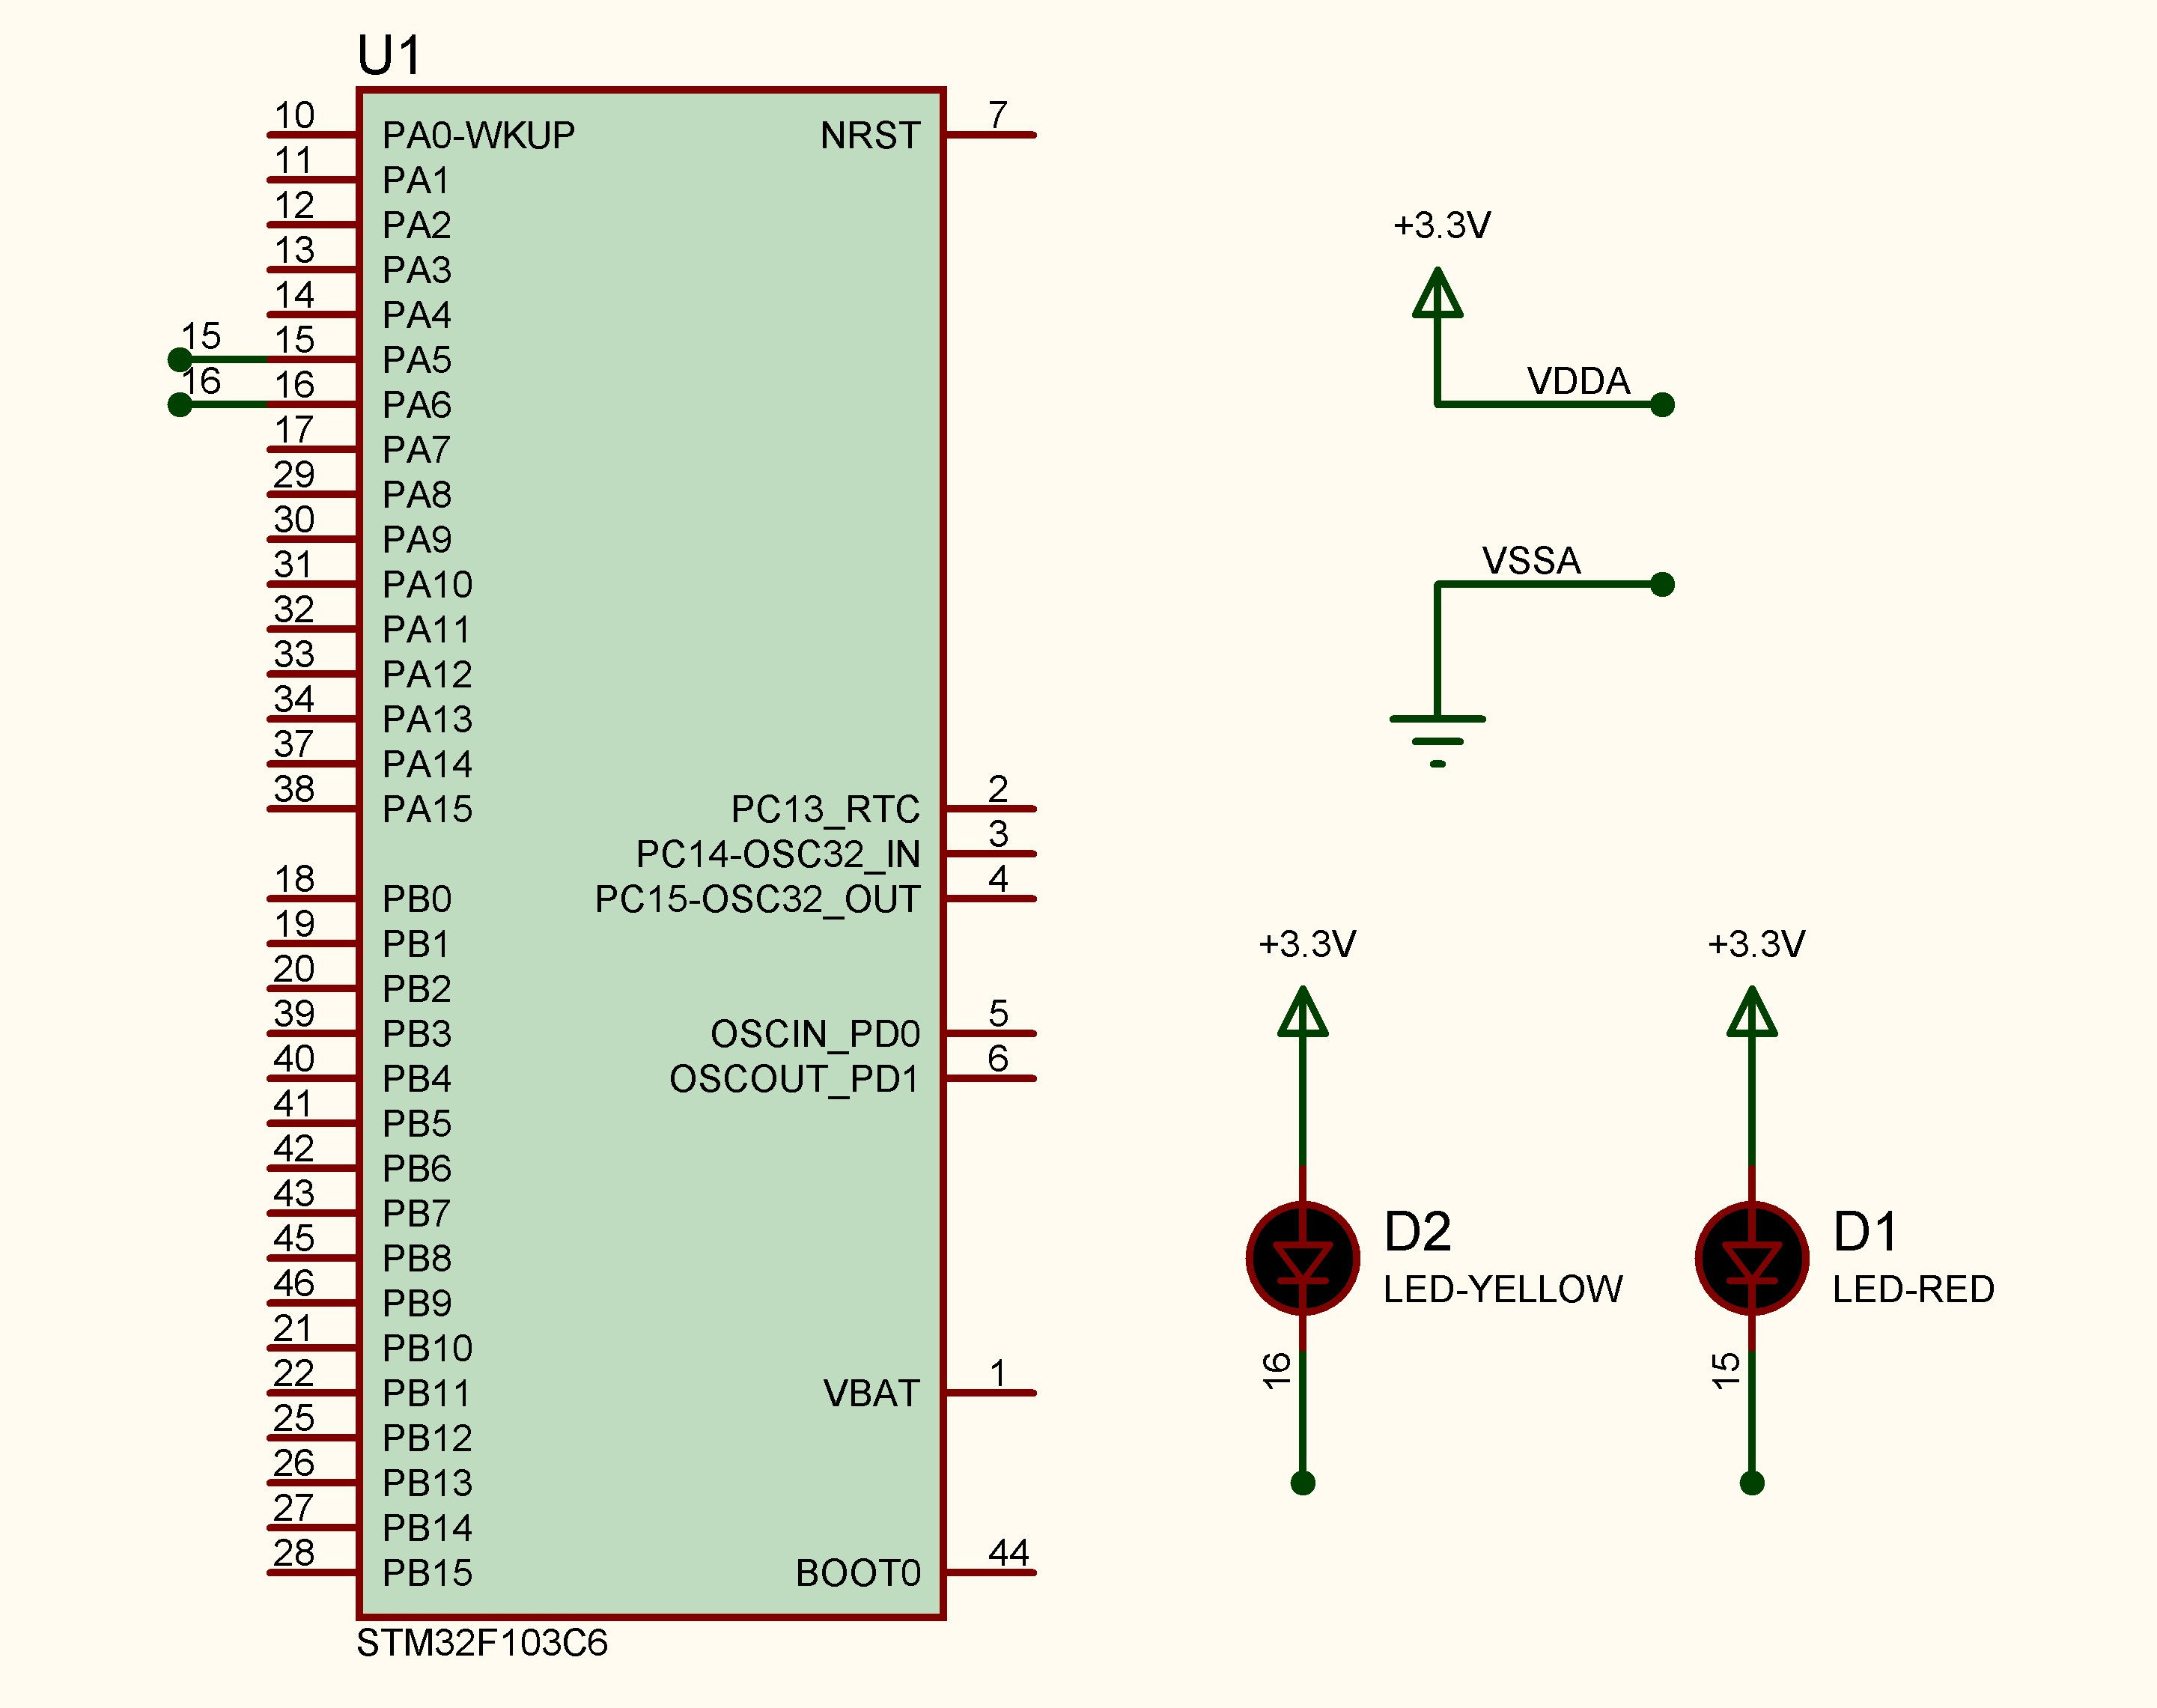
\includegraphics[width=\linewidth,height=0.82\textheight,keepaspectratio]{../../Proteus_Project/Lab1_e1/smt1.jpg}
  \vspace{0.8em}
  \caption[Exercise 1 Proteus schematic: Two-LED alternation]{Exercise 1 Proteus schematic: Two-LED alternation (\href{https://github.com/tapstoptap/microcontroller-261/raw/77b62e494c47b4563374bc61c562bf9e5548d887/Proteus_Project/Lab1_e1/Lab1_e1.pdsprj}{\texttt{Lab1\_e1.pdsprj}})}
  \label{fig:ex1_schematic}
  \vspace*{\fill}
\end{figure}
\clearpage
\restoregeometry

% ------------------------------------------------------------------------------
\subsection{Exercise 2: Three-LED Traffic Signal}
\label{subsec:ex2}
\enlargethispage{2.5\baselineskip}
\paragraph{Objective and Hardware Connection}
Construct a single-lane traffic light simulator incorporating three LEDs: Red on \texttt{PA5} (\texttt{LED\_RED\_Pin}), Yellow on \texttt{PA6}, and Green on \texttt{PA7}. The timing adheres to municipal signaling specifications: \textbf{Red: 5 seconds}, \textbf{Yellow: 2 seconds}, and \textbf{Green: 3 seconds} (total cycle $T_{cycle} = 10\,\text{s}$). The complete schematic is shown on the following dedicated page (\Cref{fig:ex2_schematic}).

\begin{table}[H]
  \centering
  \footnotesize
  \renewcommand{\arraystretch}{0.9}
  \begin{tabularx}{\linewidth}{l c c c c >{\raggedright\arraybackslash}X}
    \toprule
    \textbf{State} & \textbf{Interval} & \textbf{PA5 (Red)} & \textbf{PA6 (Yellow)} & \textbf{PA7 (Green)} & \textbf{Operational Meaning} \\
    \midrule
    \textbf{1. Stop} & 5000 ms & \textbf{RESET} (ON) & SET (OFF) & SET (OFF) & Vehicles halt; cross traffic active \\
    \textbf{2. Caution} & 2000 ms & SET (OFF) & \textbf{RESET} (ON) & SET (OFF) & Clearance before transit \\
    \textbf{3. Go} & 3000 ms & SET (OFF) & SET (OFF) & \textbf{RESET} (ON) & Transit permitted \\
    \bottomrule
  \end{tabularx}
  \caption{Exercise 2 traffic phase states and timing}
  \label{tab:ex2_states}
\end{table}

\paragraph{Firmware Implementation}
The sequential progression is implemented directly in the main loop of \texttt{Lab1\_e2/Core/Src/main.c}:

\begin{lstlisting}[caption={[Infinite loop for Exercise 2]{Infinite loop implementation for Exercise 2 (Lab1\_e2/Core/Src/main.c)}},label={lst:ex2_code},basicstyle=\fontsize{7.4pt}{8.6pt}\ttfamily,lineskip=0pt,aboveskip=1.5pt,belowskip=1.5pt]
  /* Infinite loop */
  /* USER CODE BEGIN WHILE */
  while (1)
  {
	HAL_GPIO_WritePin(GPIOA , LED_RED_Pin, GPIO_PIN_RESET);
	HAL_GPIO_WritePin(GPIOA, GPIO_PIN_6, GPIO_PIN_SET);
	HAL_GPIO_WritePin(GPIOA, GPIO_PIN_7, GPIO_PIN_SET);
	HAL_Delay(5000);
	HAL_GPIO_WritePin(GPIOA, LED_RED_Pin, GPIO_PIN_SET);
	HAL_GPIO_WritePin(GPIOA, GPIO_PIN_6, GPIO_PIN_RESET);
	HAL_GPIO_WritePin(GPIOA, GPIO_PIN_7, GPIO_PIN_SET);
	HAL_Delay(2000);
	HAL_GPIO_WritePin(GPIOA, LED_RED_Pin, GPIO_PIN_SET);
	HAL_GPIO_WritePin(GPIOA, GPIO_PIN_6, GPIO_PIN_SET);
	HAL_GPIO_WritePin(GPIOA, GPIO_PIN_7, GPIO_PIN_RESET);
    HAL_Delay(3000);
    /* USER CODE END WHILE */

    /* USER CODE BEGIN 3 */
  }
\end{lstlisting}

\paragraph{Operational Behavior}
The program drives exactly one LED low at any time, cyclically iterating through Red (5 s) $\to$ Yellow (2 s) $\to$ Green (3 s).

\clearpage
\newgeometry{left=1.5cm, right=1.5cm, top=1.5cm, bottom=1.5cm, includeheadfoot=true, headheight=35pt}
\begin{figure}[p]
  \centering
  \vspace*{\fill}
  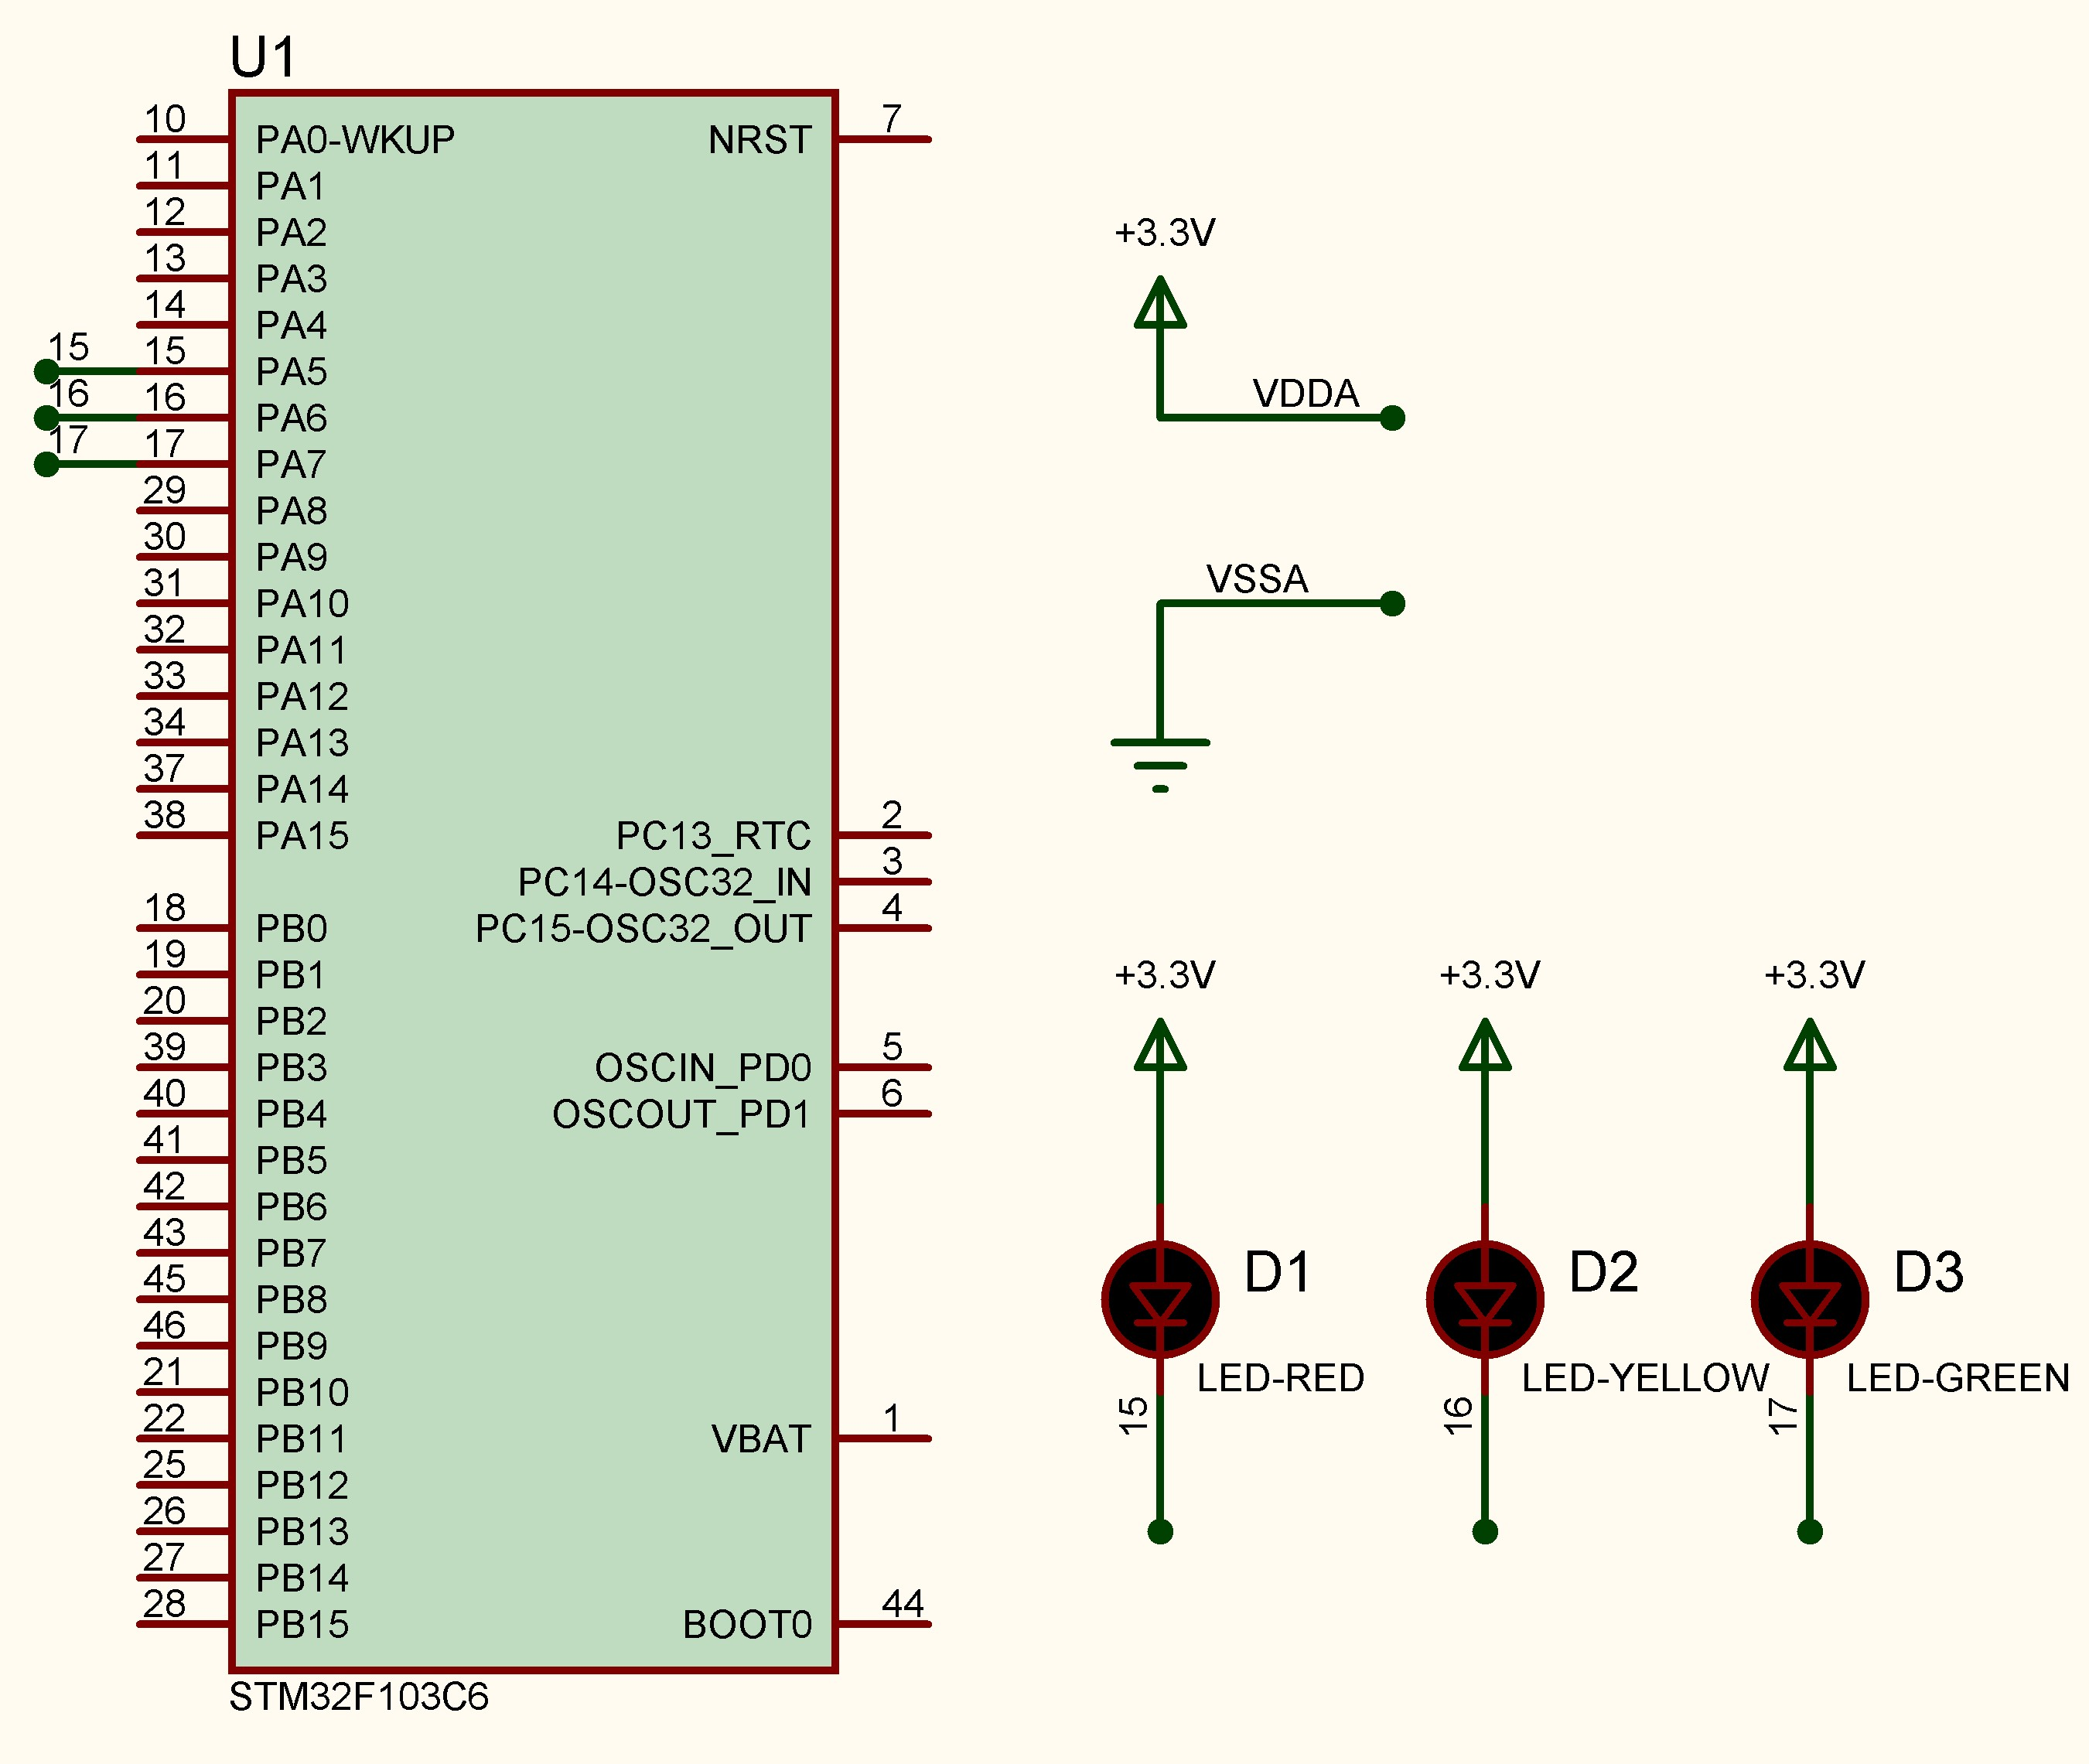
\includegraphics[width=\linewidth,height=0.82\textheight,keepaspectratio]{../../Proteus_Project/Lab1_e2/smt2.jpg}
  \vspace{0.8em}
  \caption[Exercise 2 Proteus schematic: Three-LED traffic signal]{Exercise 2 Proteus schematic: Three-LED traffic signal (\href{https://github.com/tapstoptap/microcontroller-261/raw/77b62e494c47b4563374bc61c562bf9e5548d887/Proteus_Project/Lab1_e2/Lab1_e2.pdsprj}{\texttt{Lab1\_e2.pdsprj}})}
  \label{fig:ex2_schematic}
  \vspace*{\fill}
\end{figure}
\clearpage
\restoregeometry

% ------------------------------------------------------------------------------
\subsection{Exercise 3: Four-Way 12-LED Traffic Intersection}
\label{subsec:ex3}
\enlargethispage{2.5\baselineskip}
\paragraph{Objective and Intersecting Geometry}
Expand the traffic controller to a bidirectional four-way intersection. Twelve LEDs simulate traffic lights across North, South, East, and West approaches. Opposing lanes execute synchronized operations: North and South lanes form the \textbf{NS channel}, while East and West lanes form the \textbf{WE channel}.

\paragraph{Pin Allocation and Architectural Optimization}
Rather than consuming 12 separate GPIO pins, each opposing LED pair is wired in parallel to a shared control line, utilizing 6 GPIO outputs on Port A (\Cref{tab:ex3_pins}).

\begin{table}[H]
  \centering
  \footnotesize
  \begin{tabularx}{\linewidth}{l l l c}
    \toprule
    \textbf{Signal Macro} & \textbf{Microcontroller Pin} & \textbf{Directional Assignment} & \textbf{LED Color} \\
    \midrule
    \texttt{NS\_RED\_Pin} & \texttt{GPIOA, GPIO\_PIN\_0} & North \& South Approaches & Red \\
    \texttt{NS\_YELLOW\_Pin} & \texttt{GPIOA, GPIO\_PIN\_1} & North \& South Approaches & Yellow \\
    \texttt{NS\_GREEN\_Pin} & \texttt{GPIOA, GPIO\_PIN\_2} & North \& South Approaches & Green \\
    \texttt{WE\_RED\_Pin} & \texttt{GPIOA, GPIO\_PIN\_3} & West \& East Approaches & Red \\
    \texttt{WE\_YELLOW\_Pin} & \texttt{GPIOA, GPIO\_PIN\_4} & West \& East Approaches & Yellow \\
    \texttt{WE\_GREEN\_Pin} & \texttt{GPIOA, GPIO\_PIN\_5} & West \& East Approaches & Green \\
    \bottomrule
  \end{tabularx}
  \caption{Exercise 3 GPIO pin assignments}
  \label{tab:ex3_pins}
\end{table}

\paragraph{Four-Phase State Synthesis}
To explain the clearance intervals and prevent vehicular collisions, the operational cycle is synthesized into four non-conflicting states (\Cref{tab:ex3_phases}). Note that the lab handout (page 21) introduces the 12-LED layout without mandating a state table; the table is provided here as an analytical explanation of the timing design. The green and yellow durations of one thoroughfare strictly match the red duration of the perpendicular street: $T_{\text{Red}} = T_{\text{Green}} + T_{\text{Yellow}} = 3\,\text{s} + 2\,\text{s} = 5\,\text{s}$.

\begin{table}[H]
  \centering
  \footnotesize
  \begin{tabularx}{\linewidth}{lc>{\centering\arraybackslash}p{2.6cm}>{\centering\arraybackslash}p{2.6cm}>{\raggedright\arraybackslash}X}
    \toprule
    \textbf{Phase} & \textbf{Time} & \textbf{North-South (NS)} & \textbf{West-East (WE)} & \textbf{Traffic Flow Status} \\
    \midrule
    \textbf{Phase 1} & 3 s & \textcolor{signalgreen}{\textbf{GREEN}} & \textcolor{signalred}{\textbf{RED}} & NS transit active; WE traffic stopped. \\
    \textbf{Phase 2} & 2 s & \textcolor{signalyellow}{\textbf{YELLOW}} & \textcolor{signalred}{\textbf{RED}} & NS clearance period; WE waiting. \\
    \textbf{Phase 3} & 3 s & \textcolor{signalred}{\textbf{RED}} & \textcolor{signalgreen}{\textbf{GREEN}} & WE transit active; NS traffic stopped. \\
    \textbf{Phase 4} & 2 s & \textcolor{signalred}{\textbf{RED}} & \textcolor{signalyellow}{\textbf{YELLOW}} & WE clearance period; NS waiting. \\
    \bottomrule
  \end{tabularx}
  \caption{Four-way traffic light state transition explanation}
  \label{tab:ex3_phases}
\end{table}

\clearpage
\newgeometry{left=1.5cm, right=1.5cm, top=1.5cm, bottom=1.5cm, includeheadfoot=true, headheight=35pt}
\begin{figure}[p]
  \centering
  \vspace*{\fill}
  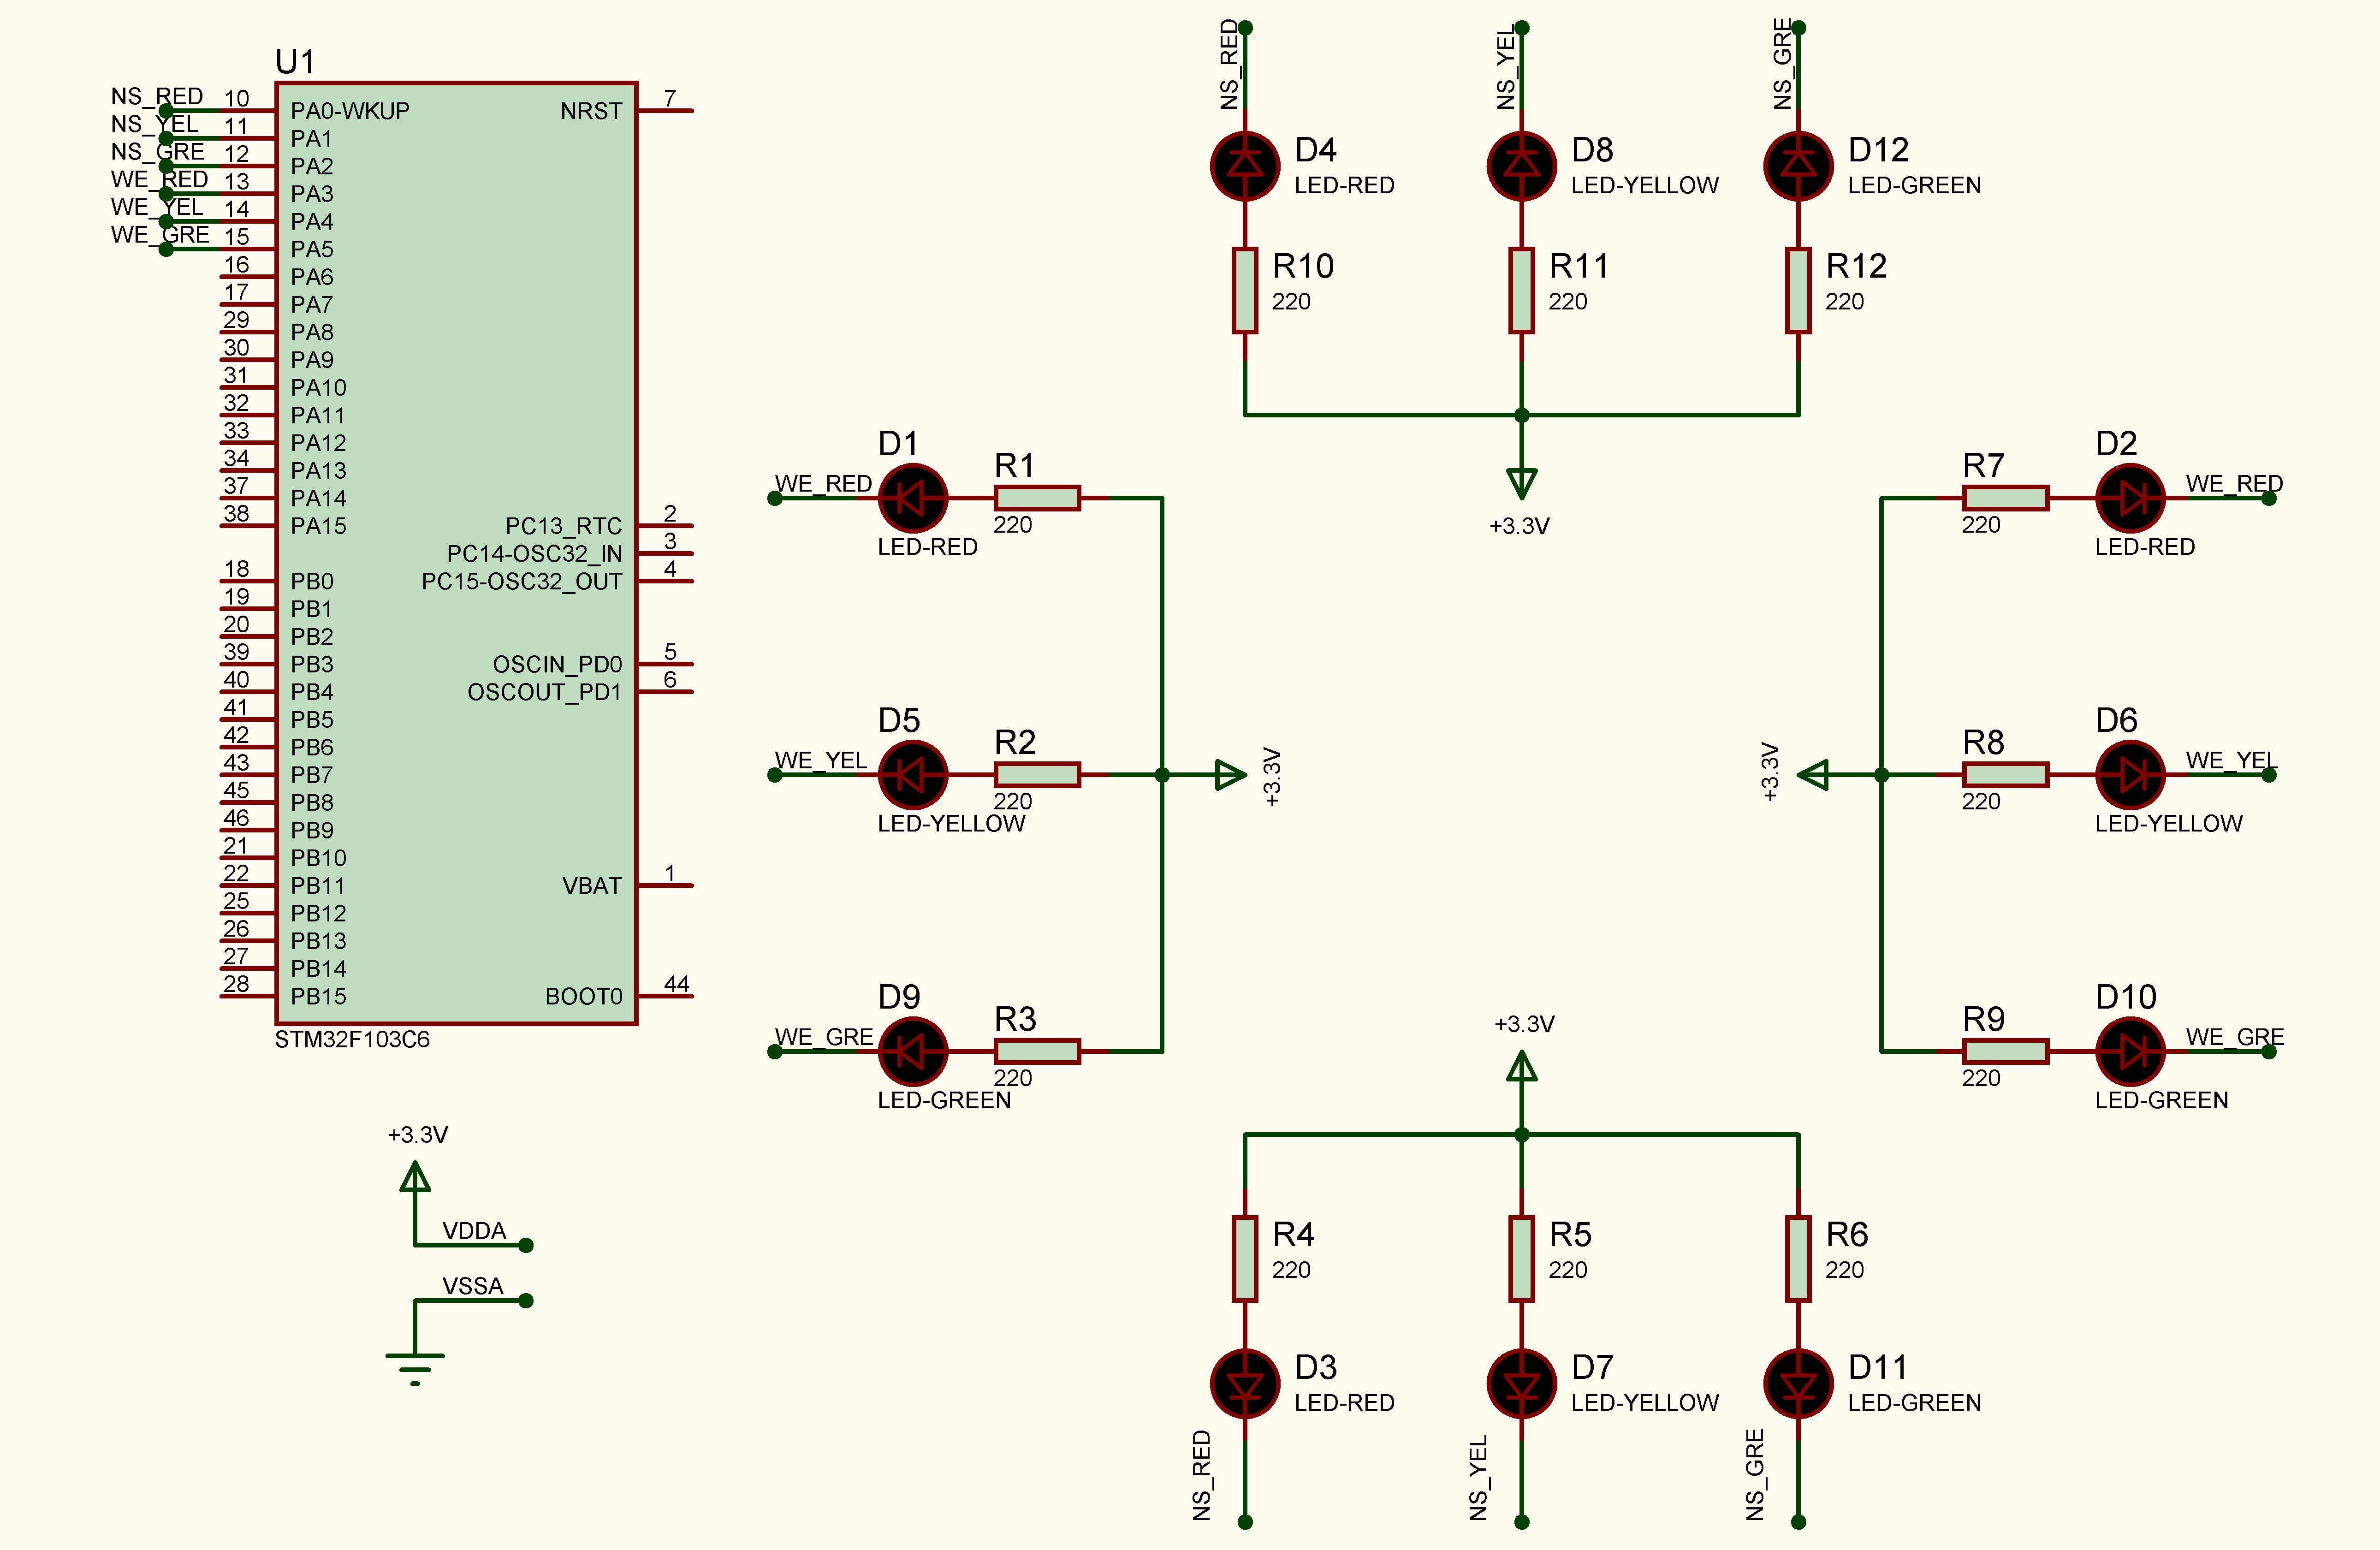
\includegraphics[width=\linewidth,height=0.82\textheight,keepaspectratio]{../../Proteus_Project/Lab1_e3/smt3.jpg}
  \vspace{0.6em}
  \caption[Exercise 3 Proteus schematic: 12-LED four-way intersection]{Exercise 3 complete Proteus schematic. Download the \href{https://github.com/tapstoptap/microcontroller-261/raw/77b62e494c47b4563374bc61c562bf9e5548d887/Proteus_Project/Lab1_e3/Lab1_e3.pdsprj}{\texttt{Lab1\_e3.pdsprj}} project for a closer view.}
  \label{fig:ex3_schematic}
  \vspace*{\fill}
\end{figure}
\clearpage
\restoregeometry

% ------------------------------------------------------------------------------
\subsection{Exercise 4: 7-Segment Common-Anode Display Decoding}
\label{subsec:ex4}
\paragraph{Display Architecture and Circuit Setup}
A single-digit 7-segment display (common-anode \texttt{7SEG-COM-ANODE}) is integrated into the system. In the Proteus schematic (\Cref{fig:ex4_schematic}, presented in full on the subsequent dedicated page), the common anode terminal is connected to the \textbf{$+3.3\,\text{V}$} power supply rail. The cathode segment pins ($a, b, c, d, e, f, g$) are wired to Port B pins \texttt{PB0} through \texttt{PB6}. The function \texttt{display7SEG(int num)} decodes numerical inputs $0 \le \text{num} \le 9$.

\paragraph{Active-Low Segment Look-Up Table}
Because the display is common-anode, pulling a GPIO pin to Logic 0 (\texttt{GPIO\_PIN\_RESET}) energizes that segment. \Cref{tab:7seg_truth} lists the segment activations and corresponding bitmask encodings.

\begin{table}[H]
  \centering
  \small
  \begin{tabularx}{\linewidth}{c ccccccc c >{\raggedright\arraybackslash}X}
    \toprule
    \textbf{Digit} & \textbf{a} & \textbf{b} & \textbf{c} & \textbf{d} & \textbf{e} & \textbf{f} & \textbf{g} & \textbf{Hex Mask} & \textbf{Active Low Pins (RESET)} \\
    \midrule
    0 & 1 & 1 & 1 & 1 & 1 & 1 & 0 & \texttt{0x3F} & PB0, PB1, PB2, PB3, PB4, PB5 \\
    1 & 0 & 1 & 1 & 0 & 0 & 0 & 0 & \texttt{0x06} & PB1, PB2 \\
    2 & 1 & 1 & 0 & 1 & 1 & 0 & 1 & \texttt{0x5B} & PB0, PB1, PB3, PB4, PB6 \\
    3 & 1 & 1 & 1 & 1 & 0 & 0 & 1 & \texttt{0x4F} & PB0, PB1, PB2, PB3, PB6 \\
    4 & 0 & 1 & 1 & 0 & 0 & 1 & 1 & \texttt{0x66} & PB1, PB2, PB5, PB6 \\
    5 & 1 & 0 & 1 & 1 & 0 & 1 & 1 & \texttt{0x6D} & PB0, PB2, PB3, PB5, PB6 \\
    6 & 1 & 0 & 1 & 1 & 1 & 1 & 1 & \texttt{0x7D} & PB0, PB2, PB3, PB4, PB5, PB6 \\
    7 & 1 & 1 & 1 & 0 & 0 & 0 & 0 & \texttt{0x07} & PB0, PB1, PB2 \\
    8 & 1 & 1 & 1 & 1 & 1 & 1 & 1 & \texttt{0x7F} & PB0, PB1, PB2, PB3, PB4, PB5, PB6 \\
    9 & 1 & 1 & 1 & 1 & 0 & 1 & 1 & \texttt{0x6F} & PB0, PB1, PB2, PB3, PB5, PB6 \\
    \bottomrule
  \end{tabularx}
  \caption{Segment encoding truth table for common-anode 7-segment display}
  \label{tab:7seg_truth}
\end{table}

\clearpage
\newgeometry{left=1.5cm, right=1.5cm, top=1.5cm, bottom=1.5cm, includeheadfoot=true, headheight=35pt}
\begin{figure}[p]
  \centering
  \vspace*{\fill}
  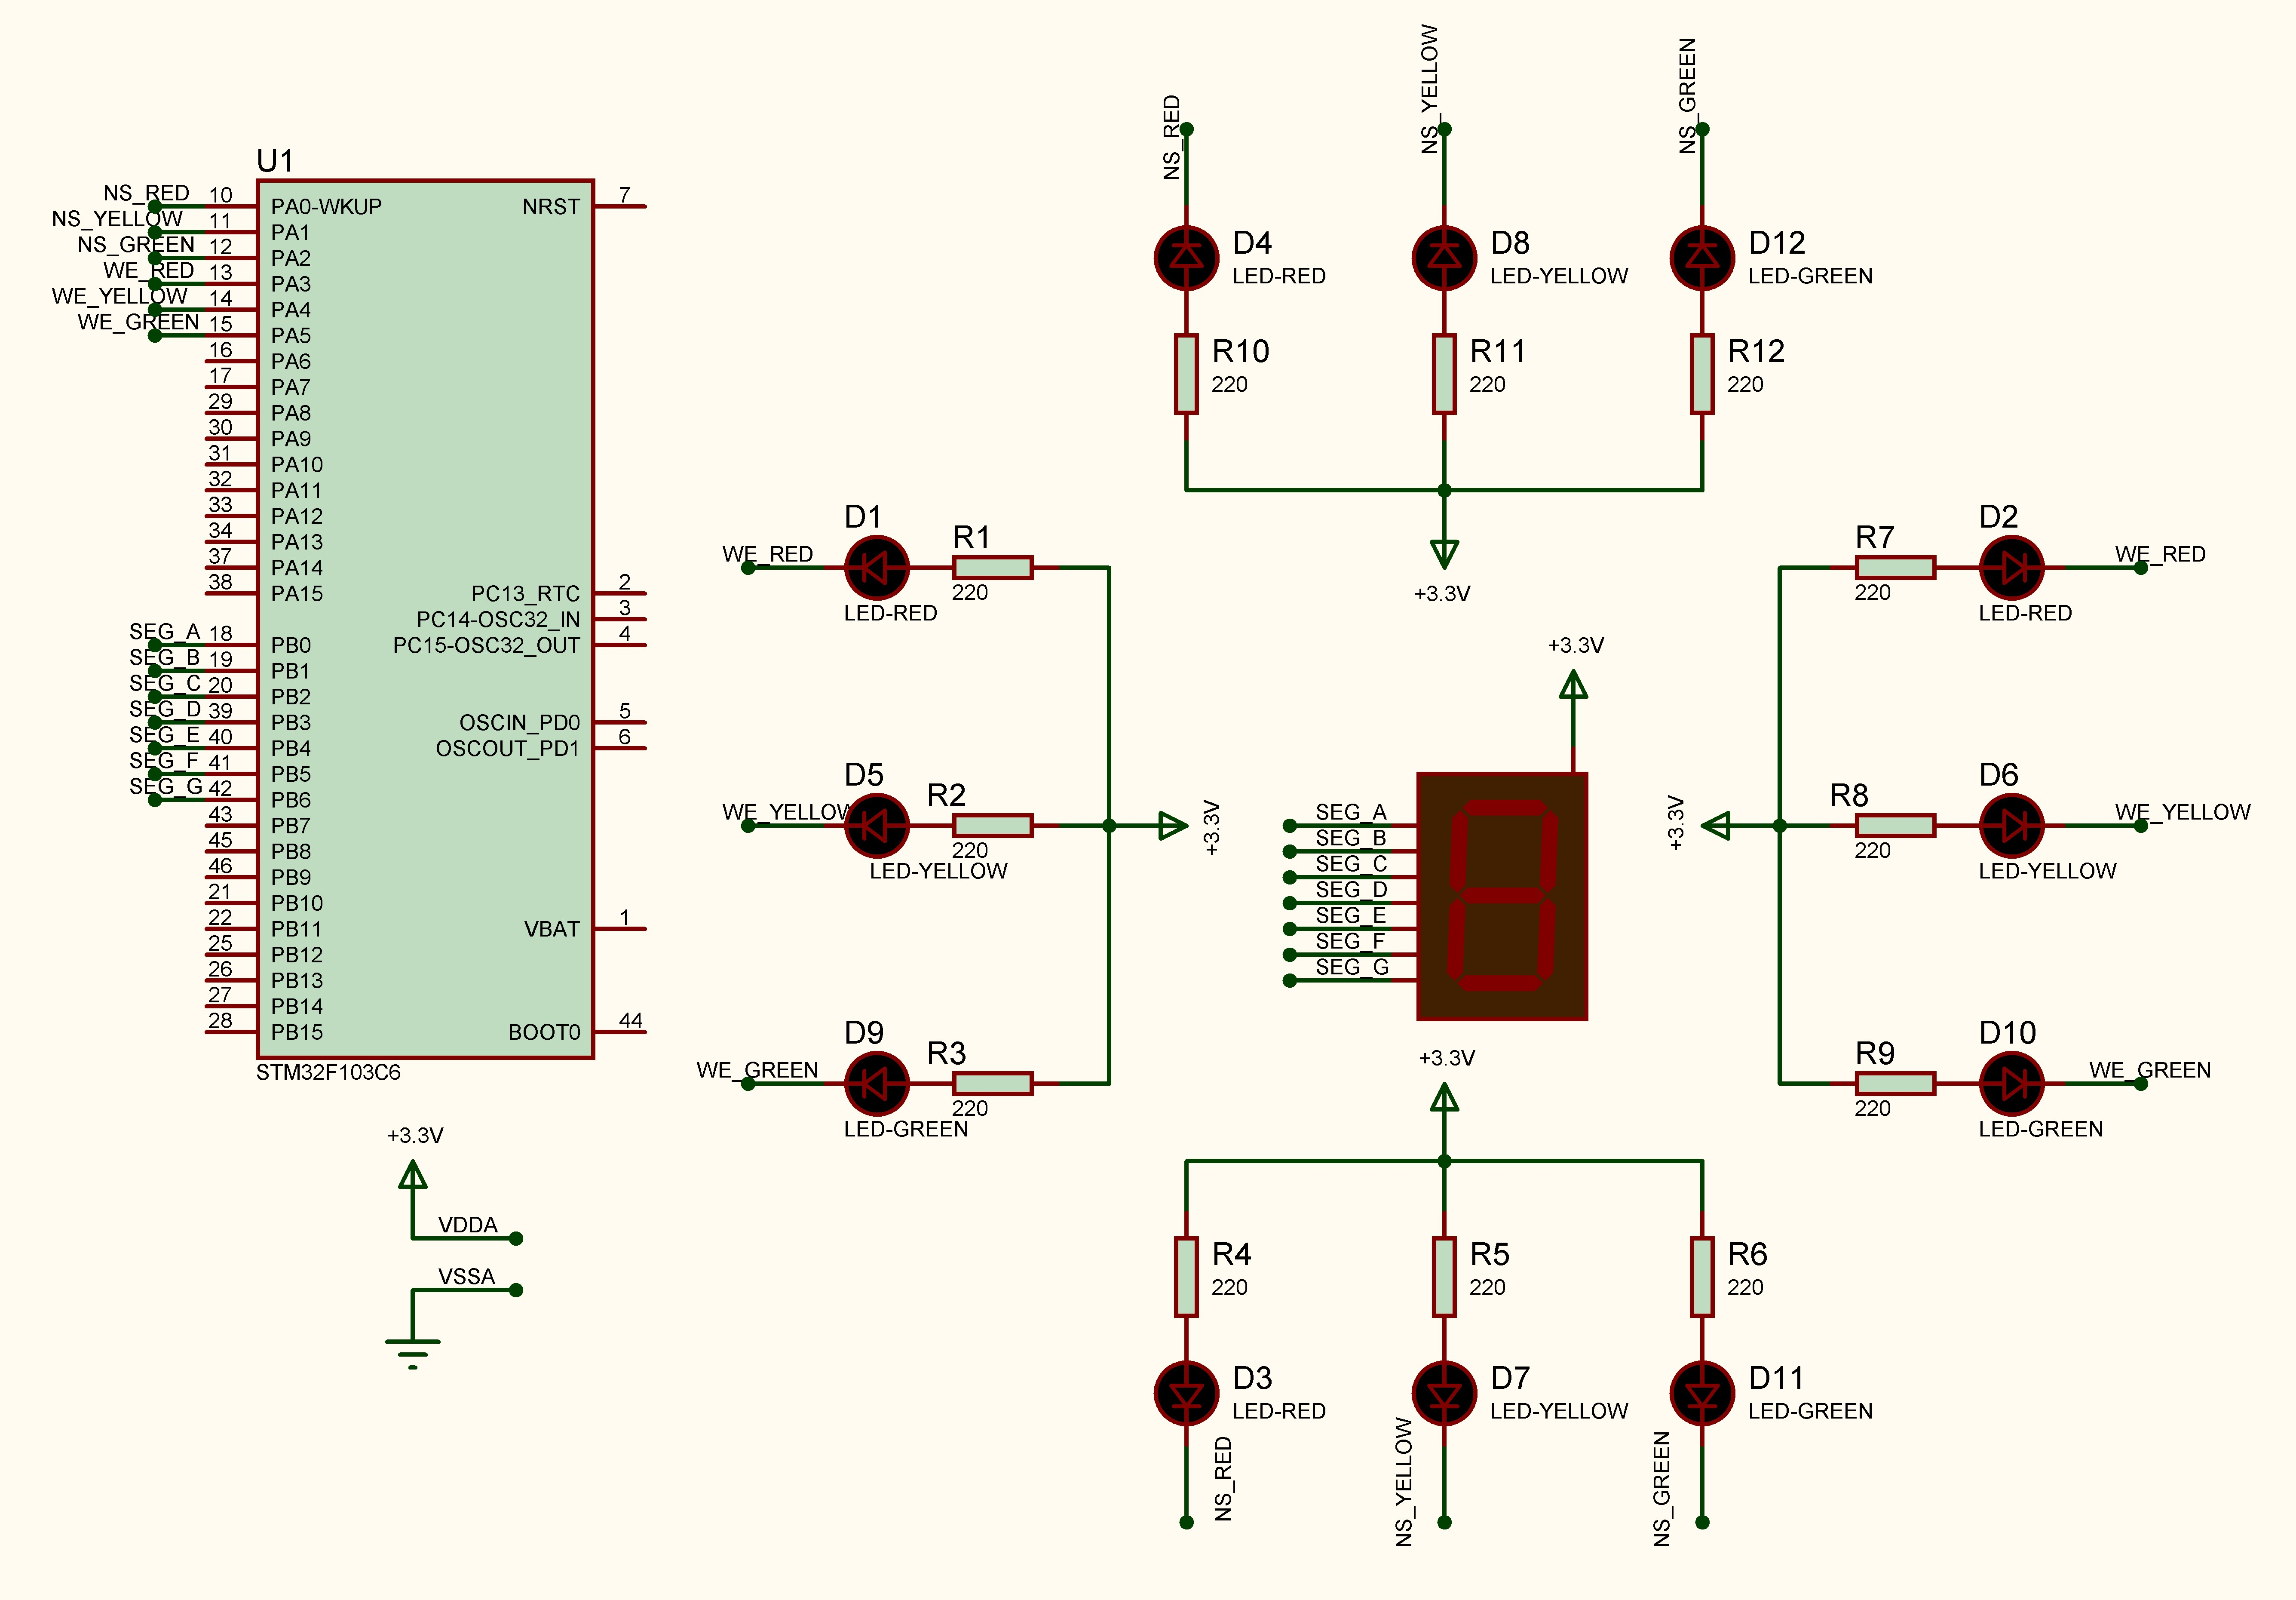
\includegraphics[width=\linewidth,height=0.82\textheight,keepaspectratio]{../../Proteus_Project/Lab1_e4/smt4.jpg}
  \vspace{0.6em}
  \caption[Exercise 4 Proteus schematic with 7-segment display]{Exercise 4 complete Proteus schematic. Download the \href{https://github.com/tapstoptap/microcontroller-261/raw/77b62e494c47b4563374bc61c562bf9e5548d887/Proteus_Project/Lab1_e4/Lab1_e4.pdsprj}{\texttt{Lab1\_e4.pdsprj}} project for a closer view.}
  \label{fig:ex4_schematic}
  \vspace*{\fill}
\end{figure}
\clearpage
\restoregeometry

\newgeometry{top=1.0cm, bottom=1.0cm, left=2.0cm, right=2.0cm, includeheadfoot=true, headheight=35pt}
\paragraph{Decoding Function Source Code}
The decoding function applies a bitmask check: if bit $n$ is 1, it emits \texttt{GPIO\_PIN\_RESET} (ON); otherwise, it emits \texttt{GPIO\_PIN\_SET} (OFF). The complete verbatim implementation from \path{Lab1_e4/Core/Src/main.c} is presented below:

\begin{lstlisting}[caption={[display7SEG() function]{Complete display7SEG(int num) implementation (Lab1\_e4/Core/Src/main.c)}},label={lst:ex4_func},basicstyle=\fontsize{7.6pt}{8.6pt}\ttfamily,lineskip=0pt,aboveskip=2pt,belowskip=2pt]
/* USER CODE BEGIN 0 */
void display7SEG(int num)
{
    /*
     * Bit order:
     * bit 0 = a
     * bit 1 = b
     * bit 2 = c
     * bit 3 = d
     * bit 4 = e
     * bit 5 = f
     * bit 6 = g
     *
     * A 1 in the table means that the segment should be ON.
     */
    static const uint8_t digit_pattern[10] =
    {
        0x3F,   // 0: a b c d e f
        0x06,   // 1:   b c
        0x5B,   // 2: a b   d e   g
        0x4F,   // 3: a b c d     g
        0x66,   // 4:   b c     f g
        0x6D,   // 5: a   c d   f g
        0x7D,   // 6: a   c d e f g
        0x07,   // 7: a b c
        0x7F,   // 8: a b c d e f g
        0x6F    // 9: a b c d   f g
    };

    if (num < 0 || num > 9)
    {
        num = 0;
    }

    uint8_t pattern = digit_pattern[num];

    HAL_GPIO_WritePin(SEG_A_GPIO_Port, SEG_A_Pin,
                      (pattern & (1U << 0)) ? GPIO_PIN_RESET : GPIO_PIN_SET);

    HAL_GPIO_WritePin(SEG_B_GPIO_Port, SEG_B_Pin,
                      (pattern & (1U << 1)) ? GPIO_PIN_RESET : GPIO_PIN_SET);

    HAL_GPIO_WritePin(SEG_C_GPIO_Port, SEG_C_Pin,
                      (pattern & (1U << 2)) ? GPIO_PIN_RESET : GPIO_PIN_SET);

    HAL_GPIO_WritePin(SEG_D_GPIO_Port, SEG_D_Pin,
                      (pattern & (1U << 3)) ? GPIO_PIN_RESET : GPIO_PIN_SET);

    HAL_GPIO_WritePin(SEG_E_GPIO_Port, SEG_E_Pin,
                      (pattern & (1U << 4)) ? GPIO_PIN_RESET : GPIO_PIN_SET);

    HAL_GPIO_WritePin(SEG_F_GPIO_Port, SEG_F_Pin,
                      (pattern & (1U << 5)) ? GPIO_PIN_RESET : GPIO_PIN_SET);

    HAL_GPIO_WritePin(SEG_G_GPIO_Port, SEG_G_Pin,
                      (pattern & (1U << 6)) ? GPIO_PIN_RESET : GPIO_PIN_SET);
}
/* USER CODE END 0 */
\end{lstlisting}
\clearpage
\restoregeometry

% ------------------------------------------------------------------------------
\subsection{Exercise 5: Integrated Traffic Light with Countdown Display}
\label{subsec:ex5}
\paragraph{Objective and Operational Sequence}
Integrate the 7-segment display with the four-way traffic controller to present real-time countdown seconds for active traffic phases. In strict accordance with the lab handout (page 22), only the integration source code is required.

Inspection of the actual source implementation in \texttt{Lab1\_e5/Core/Src/main.c} reveals the exact operational sequence:
\begin{itemize}[leftmargin=*,itemsep=1pt]
  \item \textbf{Phase 1 (3 seconds):} \textbf{North--South RED} (\texttt{NS\_RED\_Pin} asserted low) and \textbf{West--East GREEN} (\texttt{WE\_GREEN\_Pin} asserted low). The helper function calls \texttt{runPhase(3)}, displaying countdown values 3, 2, 1 on the 7-segment display.
  \item \textbf{Phase 2 (2 seconds):} \textbf{North--South RED} (continued for 2 more seconds, completing a 5-second red interval) and \textbf{West--East YELLOW} (\texttt{WE\_YELLOW\_Pin} asserted low). The helper function calls \texttt{runPhase(2)}, displaying countdown values 2, 1.
  \item \textbf{Phase 3 (3 seconds):} \textbf{West--East RED} (\texttt{WE\_RED\_Pin} asserted low) and \textbf{North--South GREEN} (\texttt{NS\_GREEN\_Pin} asserted low). The helper function calls \texttt{runPhase(3)}, displaying countdown values 3, 2, 1.
  \item \textbf{Phase 4 (2 seconds):} \textbf{West--East RED} (continued for 2 more seconds, completing a 5-second red interval) and \textbf{North--South YELLOW} (\texttt{NS\_YELLOW\_Pin} asserted low). The helper function calls \texttt{runPhase(2)}, displaying countdown values 2, 1.
\end{itemize}

\paragraph{Verbatim Implementation Source Code}
The listings below present the complete, verbatim source code from \texttt{Lab1\_e5/Core/Src/main.c}:

\begin{lstlisting}[caption={[Countdown helper function runPhase()]{Countdown driver function runPhase() (Lab1\_e5/Core/Src/main.c)}},label={lst:ex5_runphase}]
void runPhase(uint8_t seconds)
{
    for (int time_left = seconds; time_left > 0; time_left--)
    {
        display7SEG(time_left);
        HAL_Delay(1000);
    }
}
/* USER CODE END 0 */
\end{lstlisting}

\clearpage
\newgeometry{top=1.0cm, bottom=1.0cm, left=2.0cm, right=2.0cm, includeheadfoot=true, headheight=35pt}
\begin{lstlisting}[caption={[Integrated traffic countdown while loop]{Integrated traffic countdown while (1) loop (Lab1\_e5/Core/Src/main.c)}},label={lst:ex5_while},basicstyle=\fontsize{6.4pt}{7.2pt}\ttfamily,lineskip=0pt,aboveskip=1pt,belowskip=1pt]
  /* Infinite loop */
  /* USER CODE BEGIN WHILE */
  while (1)
  {
      /*
       * Phase 1: NS_RED (3s) & WE_GREEN (3s)
       * North/South: RED
       * West/East: GREEN
       */
      HAL_GPIO_WritePin(NS_RED_GPIO_Port,
                        NS_RED_Pin,
                        GPIO_PIN_RESET);

      HAL_GPIO_WritePin(NS_YELLOW_GPIO_Port,
                        NS_YELLOW_Pin,
                        GPIO_PIN_SET);

      HAL_GPIO_WritePin(NS_GREEN_GPIO_Port,
                        NS_GREEN_Pin,
                        GPIO_PIN_SET);

      HAL_GPIO_WritePin(WE_RED_GPIO_Port,
                        WE_RED_Pin,
                        GPIO_PIN_SET);

      HAL_GPIO_WritePin(WE_YELLOW_GPIO_Port,
                        WE_YELLOW_Pin,
                        GPIO_PIN_SET);

      HAL_GPIO_WritePin(WE_GREEN_GPIO_Port,
                        WE_GREEN_Pin,
                        GPIO_PIN_RESET);

      runPhase(3);


      /*
       * Phase 2: NS_RED (continued for 2s, total 5s) & WE_YELLOW (2s)
       * North/South: RED
       * West/East: YELLOW
       */
      HAL_GPIO_WritePin(NS_RED_GPIO_Port,
                        NS_RED_Pin,
                        GPIO_PIN_RESET);

      HAL_GPIO_WritePin(NS_YELLOW_GPIO_Port,
                        NS_YELLOW_Pin,
                        GPIO_PIN_SET);

      HAL_GPIO_WritePin(NS_GREEN_GPIO_Port,
                        NS_GREEN_Pin,
                        GPIO_PIN_SET);

      HAL_GPIO_WritePin(WE_RED_GPIO_Port,
                        WE_RED_Pin,
                        GPIO_PIN_SET);

      HAL_GPIO_WritePin(WE_YELLOW_GPIO_Port,
                        WE_YELLOW_Pin,
                        GPIO_PIN_RESET);

      HAL_GPIO_WritePin(WE_GREEN_GPIO_Port,
                        WE_GREEN_Pin,
                        GPIO_PIN_SET);

      runPhase(2);


      /*
       * Phase 3: WE_RED (3s) & NS_GREEN (3s)
       * North/South: GREEN
       * West/East: RED
       */
      HAL_GPIO_WritePin(NS_RED_GPIO_Port,
                        NS_RED_Pin,
                        GPIO_PIN_SET);

      HAL_GPIO_WritePin(NS_YELLOW_GPIO_Port,
                        NS_YELLOW_Pin,
                        GPIO_PIN_SET);

      HAL_GPIO_WritePin(NS_GREEN_GPIO_Port,
                        NS_GREEN_Pin,
                        GPIO_PIN_RESET);

      HAL_GPIO_WritePin(WE_RED_GPIO_Port,
                        WE_RED_Pin,
                        GPIO_PIN_RESET);

      HAL_GPIO_WritePin(WE_YELLOW_GPIO_Port,
                        WE_YELLOW_Pin,
                        GPIO_PIN_SET);

      HAL_GPIO_WritePin(WE_GREEN_GPIO_Port,
                        WE_GREEN_Pin,
                        GPIO_PIN_SET);

      runPhase(3);


      /*
       * Phase 4: WE_RED (continued for 2s, total 5s) & NS_YELLOW (2s)
       * North/South: YELLOW
       * West/East: RED
       */
      HAL_GPIO_WritePin(NS_RED_GPIO_Port,
                        NS_RED_Pin,
                        GPIO_PIN_SET);

      HAL_GPIO_WritePin(NS_YELLOW_GPIO_Port,
                        NS_YELLOW_Pin,
                        GPIO_PIN_RESET);

      HAL_GPIO_WritePin(NS_GREEN_GPIO_Port,
                        NS_GREEN_Pin,
                        GPIO_PIN_SET);

      HAL_GPIO_WritePin(WE_RED_GPIO_Port,
                        WE_RED_Pin,
                        GPIO_PIN_RESET);

      HAL_GPIO_WritePin(WE_YELLOW_GPIO_Port,
                        WE_YELLOW_Pin,
                        GPIO_PIN_SET);

      HAL_GPIO_WritePin(WE_GREEN_GPIO_Port,
                        WE_GREEN_Pin,
                        GPIO_PIN_SET);

      runPhase(2);
  }
  /* USER CODE END WHILE */
\end{lstlisting}

\paragraph{Operational Behavior}
The implementation delivers a continuous, repeating 10-second traffic cycle. In Phase 1, West--East traffic proceeds under green while North--South halts; the countdown decrements $3 \to 2 \to 1$. In Phase 2, West--East warns vehicles with yellow ($2 \to 1$) while North--South remains red. In Phase 3, North--South proceeds under green ($3 \to 2 \to 1$) while West--East stops. In Phase 4, North--South clears under yellow ($2 \to 1$) while West--East remains red. All phase durations and display outputs match the C code logic.

\clearpage
\restoregeometry

% ==============================================================================
% SECTION 3
% ==============================================================================
\section{Analog Clock Simulation with 12 LEDs (Exercises 6--10)}
\label{sec:ex6to10}

\subsection{Exercise 6: 12-LED Clock Dial Interface and Sequential Test}
\label{subsec:ex6}
\paragraph{Objective and Hardware Setup}
Simulate an analog clock dial using 12 discrete LEDs arranged radially. In the Proteus schematic (\Cref{fig:ex6_schematic}, presented in full on the subsequent dedicated page), the LEDs connect to Port A pins \texttt{PA4} through \texttt{PA15}. A sequential testing program verifies the electrical connections by turning on each individual LED in sequence with a 500 ms dwell time.

\paragraph{Dial LED Pin Allocations and Sequential Sweep Order}
Table \ref{tab:ex6_dial_pins} details the radial LED connection topology across Port A and the activation sequence executed by the testing firmware.

\begin{table}[H]
  \centering
  \footnotesize
  \begin{tabularx}{\linewidth}{c c c >{\raggedright\arraybackslash}X}
    \toprule
    \textbf{Dial Numeral} & \textbf{LED Designator} & \textbf{MCU Port Pin} & \textbf{Sequential Verification Step} \\
    \midrule
    12 & \texttt{D1}  & \texttt{GPIOA, GPIO\_PIN\_4}  & Step 1: Active-low pulse (500 ms) \\
    1  & \texttt{D2}  & \texttt{GPIOA, GPIO\_PIN\_5}  & Step 2: Active-low pulse (500 ms) \\
    2  & \texttt{D3}  & \texttt{GPIOA, GPIO\_PIN\_6}  & Step 3: Active-low pulse (500 ms) \\
    3  & \texttt{D4}  & \texttt{GPIOA, GPIO\_PIN\_7}  & Step 4: Active-low pulse (500 ms) \\
    4  & \texttt{D5}  & \texttt{GPIOA, GPIO\_PIN\_8}  & Step 5: Active-low pulse (500 ms) \\
    5  & \texttt{D6}  & \texttt{GPIOA, GPIO\_PIN\_9}  & Step 6: Active-low pulse (500 ms) \\
    6  & \texttt{D7}  & \texttt{GPIOA, GPIO\_PIN\_10} & Step 7: Active-low pulse (500 ms) \\
    7  & \texttt{D8}  & \texttt{GPIOA, GPIO\_PIN\_11} & Step 8: Active-low pulse (500 ms) \\
    8  & \texttt{D9}  & \texttt{GPIOA, GPIO\_PIN\_12} & Step 9: Active-low pulse (500 ms) \\
    9  & \texttt{D10} & \texttt{GPIOA, GPIO\_PIN\_13} & Step 10: Active-low pulse (500 ms) \\
    10 & \texttt{D11} & \texttt{GPIOA, GPIO\_PIN\_14} & Step 11: Active-low pulse (500 ms) \\
    11 & \texttt{D12} & \texttt{GPIOA, GPIO\_PIN\_15} & Step 12: Active-low pulse (500 ms) \\
    \bottomrule
  \end{tabularx}
  \caption{Exercise 6 dial LED pin assignments and sweep sequence}
  \label{tab:ex6_dial_pins}
\end{table}

\clearpage
\newgeometry{left=1.5cm, right=1.5cm, top=1.5cm, bottom=1.5cm, includeheadfoot=true, headheight=35pt}
\begin{figure}[p]
  \centering
  \vspace*{\fill}
  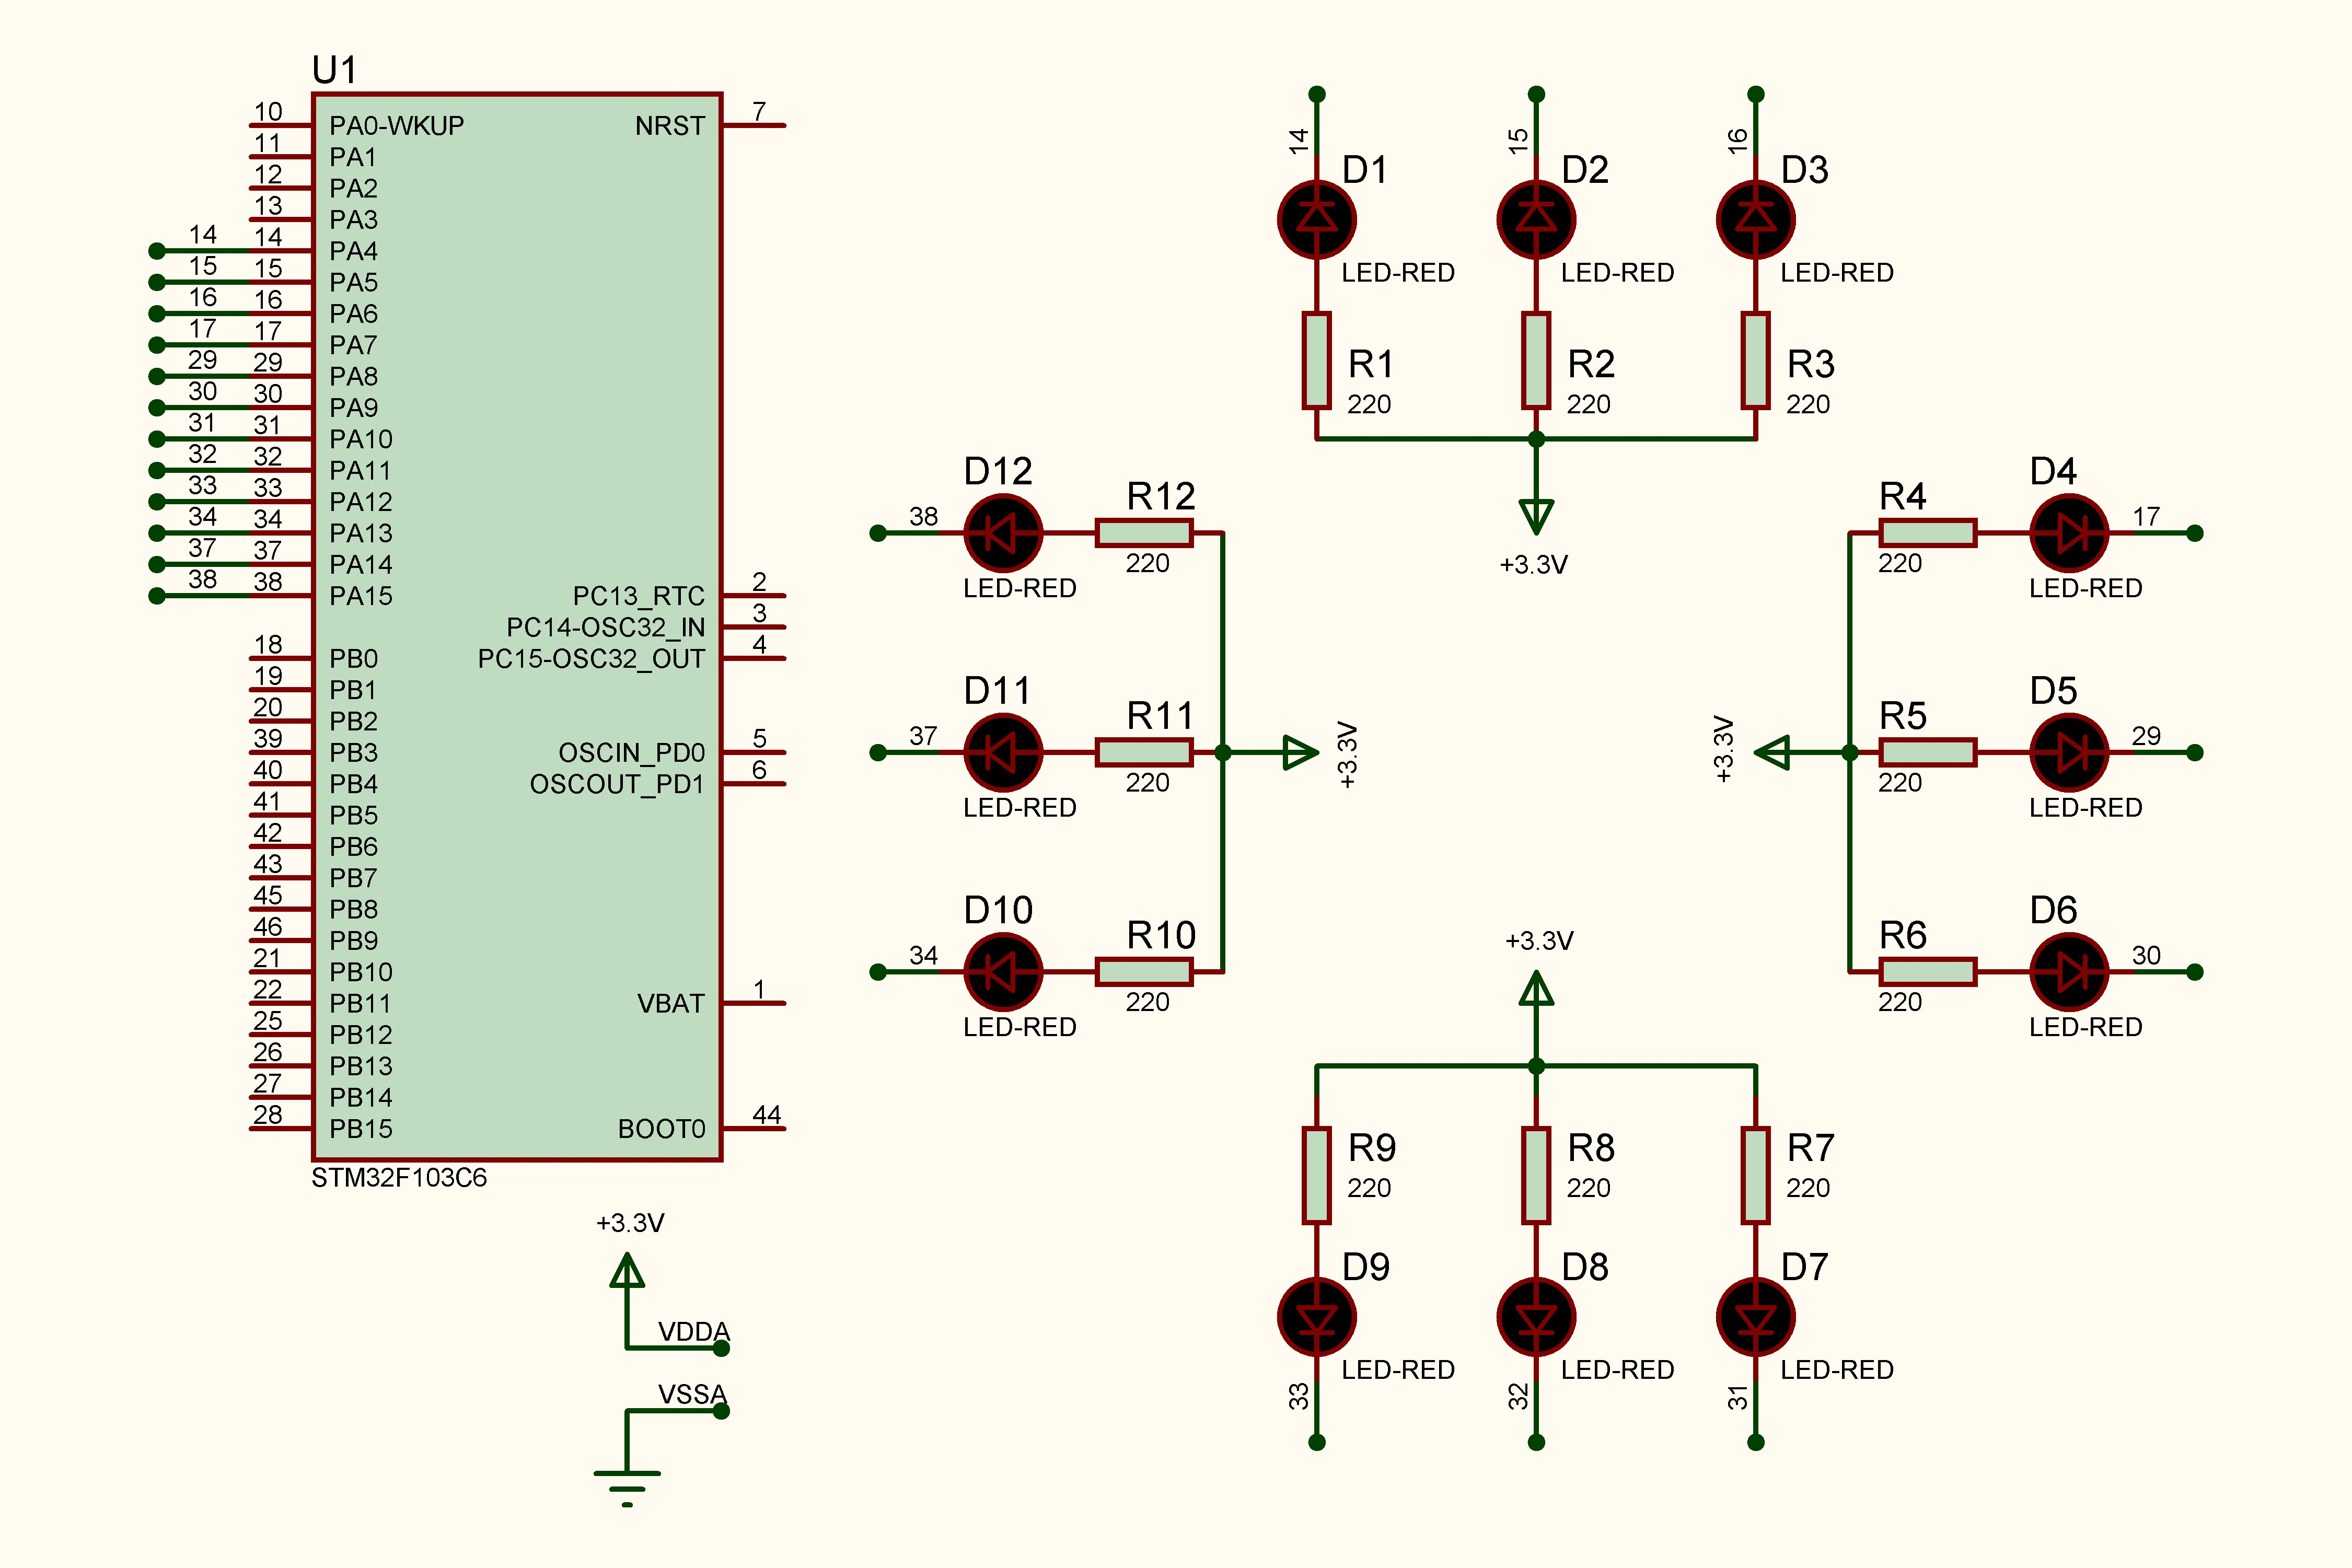
\includegraphics[width=\linewidth,height=0.82\textheight,keepaspectratio]{../../Proteus_Project/Lab1_e6/smt6.jpg}
  \vspace{0.6em}
  \caption[Exercise 6 Proteus schematic: 12-LED analog clock on PA4--PA15]{Exercise 6 complete Proteus schematic. Download the \href{https://github.com/tapstoptap/microcontroller-261/raw/77b62e494c47b4563374bc61c562bf9e5548d887/Proteus_Project/Lab1_e6/Lab1_e6.pdsprj}{\texttt{Lab1\_e6.pdsprj}} project for a closer view.}
  \label{fig:ex6_schematic}
  \vspace*{\fill}
\end{figure}
\clearpage
\restoregeometry

\newgeometry{top=1.0cm, bottom=1.0cm, left=2.0cm, right=2.0cm, includeheadfoot=true, headheight=35pt}
\paragraph{Sequential Test Program Implementation}
The listing below reproduces the verbatim implementation from \path{Lab1_e6/Core/Src/main.c}. Rather than using an array loop, the source code executes explicit sequential HAL writes: first setting all 12 pins high (\texttt{GPIO\_PIN\_SET}) to extinguish the display, then pulsing each pin low (\texttt{GPIO\_PIN\_RESET}) for 500 ms:

\begin{lstlisting}[caption={[Sequential LED test program]{Sequential LED test program (Lab1\_e6/Core/Src/main.c)}},label={lst:ex6_code},basicstyle=\fontsize{6.4pt}{7.0pt}\ttfamily,lineskip=0pt,aboveskip=1pt,belowskip=1pt]
  /* Infinite loop */
  /* USER CODE BEGIN WHILE */
  while (1)
  {
      // Turn all 12 LEDs OFF
      HAL_GPIO_WritePin(GPIOA, GPIO_PIN_4,  GPIO_PIN_SET);
      HAL_GPIO_WritePin(GPIOA, GPIO_PIN_5,  GPIO_PIN_SET);
      HAL_GPIO_WritePin(GPIOA, GPIO_PIN_6,  GPIO_PIN_SET);
      HAL_GPIO_WritePin(GPIOA, GPIO_PIN_7,  GPIO_PIN_SET);
      HAL_GPIO_WritePin(GPIOA, GPIO_PIN_8,  GPIO_PIN_SET);
      HAL_GPIO_WritePin(GPIOA, GPIO_PIN_9,  GPIO_PIN_SET);
      HAL_GPIO_WritePin(GPIOA, GPIO_PIN_10, GPIO_PIN_SET);
      HAL_GPIO_WritePin(GPIOA, GPIO_PIN_11, GPIO_PIN_SET);
      HAL_GPIO_WritePin(GPIOA, GPIO_PIN_12, GPIO_PIN_SET);
      HAL_GPIO_WritePin(GPIOA, GPIO_PIN_13, GPIO_PIN_SET);
      HAL_GPIO_WritePin(GPIOA, GPIO_PIN_14, GPIO_PIN_SET);
      HAL_GPIO_WritePin(GPIOA, GPIO_PIN_15, GPIO_PIN_SET);

      // Turn on one LED at a time
      HAL_GPIO_WritePin(GPIOA, GPIO_PIN_4, GPIO_PIN_RESET);
      HAL_Delay(500);

      HAL_GPIO_WritePin(GPIOA, GPIO_PIN_4, GPIO_PIN_SET);
      HAL_GPIO_WritePin(GPIOA, GPIO_PIN_5, GPIO_PIN_RESET);
      HAL_Delay(500);

      HAL_GPIO_WritePin(GPIOA, GPIO_PIN_5, GPIO_PIN_SET);
      HAL_GPIO_WritePin(GPIOA, GPIO_PIN_6, GPIO_PIN_RESET);
      HAL_Delay(500);

      HAL_GPIO_WritePin(GPIOA, GPIO_PIN_6, GPIO_PIN_SET);
      HAL_GPIO_WritePin(GPIOA, GPIO_PIN_7, GPIO_PIN_RESET);
      HAL_Delay(500);

      HAL_GPIO_WritePin(GPIOA, GPIO_PIN_7, GPIO_PIN_SET);
      HAL_GPIO_WritePin(GPIOA, GPIO_PIN_8, GPIO_PIN_RESET);
      HAL_Delay(500);

      HAL_GPIO_WritePin(GPIOA, GPIO_PIN_8, GPIO_PIN_SET);
      HAL_GPIO_WritePin(GPIOA, GPIO_PIN_9, GPIO_PIN_RESET);
      HAL_Delay(500);

      HAL_GPIO_WritePin(GPIOA, GPIO_PIN_9, GPIO_PIN_SET);
      HAL_GPIO_WritePin(GPIOA, GPIO_PIN_10, GPIO_PIN_RESET);
      HAL_Delay(500);

      HAL_GPIO_WritePin(GPIOA, GPIO_PIN_10, GPIO_PIN_SET);
      HAL_GPIO_WritePin(GPIOA, GPIO_PIN_11, GPIO_PIN_RESET);
      HAL_Delay(500);

      HAL_GPIO_WritePin(GPIOA, GPIO_PIN_11, GPIO_PIN_SET);
      HAL_GPIO_WritePin(GPIOA, GPIO_PIN_12, GPIO_PIN_RESET);
      HAL_Delay(500);

      HAL_GPIO_WritePin(GPIOA, GPIO_PIN_12, GPIO_PIN_SET);
      HAL_GPIO_WritePin(GPIOA, GPIO_PIN_13, GPIO_PIN_RESET);
      HAL_Delay(500);

      HAL_GPIO_WritePin(GPIOA, GPIO_PIN_13, GPIO_PIN_SET);
      HAL_GPIO_WritePin(GPIOA, GPIO_PIN_14, GPIO_PIN_RESET);
      HAL_Delay(500);

      HAL_GPIO_WritePin(GPIOA, GPIO_PIN_14, GPIO_PIN_SET);
      HAL_GPIO_WritePin(GPIOA, GPIO_PIN_15, GPIO_PIN_RESET);
      HAL_Delay(500);

      HAL_GPIO_WritePin(GPIOA, GPIO_PIN_15, GPIO_PIN_SET);
  }
  /* USER CODE END WHILE */
\end{lstlisting}
% ------------------------------------------------------------------------------
\subsection{Exercise 7: Complete \texttt{clearAllClock()} Implementation}
\label{subsec:ex7}
\paragraph{Objective and Helper Logic}
Implement a dedicated helper function to clear all 12 clock LEDs simultaneously. In active-low configuration, setting the pin to Logic 1 opens the circuit by equalizing anode and cathode potentials. The listing below presents the verbatim implementation from \path{Lab1_e7/Core/Src/main.c}:

\begin{lstlisting}[caption={[clearAllClock() function]{Complete clearAllClock() implementation (Lab1\_e7/Core/Src/main.c)}},label={lst:ex7_func},basicstyle=\fontsize{6.6pt}{7.3pt}\ttfamily,lineskip=0pt,aboveskip=0pt,belowskip=0pt]
/* USER CODE BEGIN 0 */
void clearAllClock(void)
{
    HAL_GPIO_WritePin(
        GPIOA,
        GPIO_PIN_4  |
        GPIO_PIN_5  |
        GPIO_PIN_6  |
        GPIO_PIN_7  |
        GPIO_PIN_8  |
        GPIO_PIN_9  |
        GPIO_PIN_10 |
        GPIO_PIN_11 |
        GPIO_PIN_12 |
        GPIO_PIN_13 |
        GPIO_PIN_14 |
        GPIO_PIN_15,
        GPIO_PIN_SET
    );
}
/* USER CODE END 0 */
\end{lstlisting}

\noindent By performing a bitwise OR of pin bitmasks \texttt{0x0010} through \texttt{0x8000} (resulting in \texttt{0xFFF0}), the HAL driver updates all 12 pins in a single register write to \texttt{GPIOA->BSRR}.

\vspace{-0.4em}
% ------------------------------------------------------------------------------
\subsection{Exercise 8: Complete \texttt{setNumberOnClock(int num)} Implementation}
\label{subsec:ex8}
\paragraph{Objective and Implementation}
Implement \texttt{setNumberOnClock(int num)} to selectively turn on the single LED corresponding to input index $0 \le \text{num} \le 11$. The function clears all other LEDs prior to asserting the target pin low. The listing below presents the verbatim implementation from \path{Lab1_e8/Core/Src/main.c}:

\begin{lstlisting}[caption={[setNumberOnClock() function]{Complete setNumberOnClock(int num) implementation (Lab1\_e8/Core/Src/main.c)}},label={lst:ex8_func},basicstyle=\fontsize{6.6pt}{7.3pt}\ttfamily,lineskip=0pt,aboveskip=0pt,belowskip=0pt]
/* USER CODE BEGIN 0 */
void setNumberOnClock(int num)
{
    static const uint16_t clock_pins[12] =
    {
        GPIO_PIN_4,
        GPIO_PIN_5,
        GPIO_PIN_6,
        GPIO_PIN_7,
        GPIO_PIN_8,
        GPIO_PIN_9,
        GPIO_PIN_10,
        GPIO_PIN_11,
        GPIO_PIN_12,
        GPIO_PIN_13,
        GPIO_PIN_14,
        GPIO_PIN_15
    };

    // Turn off all LEDs first
    clearAllClock();

    // Accept only numbers from 0 to 11
    if (num >= 0 && num < 12)
    {
        // Active-low LED: RESET turns the selected LED on
        HAL_GPIO_WritePin(GPIOA,
                          clock_pins[num],
                          GPIO_PIN_RESET);
    }
}
/* USER CODE END 0 */
\end{lstlisting}

% ------------------------------------------------------------------------------
\subsection{Exercise 9: Complete \texttt{clearNumberOnClock(int num)} Implementation}
\label{subsec:ex9}
\paragraph{Objective and Implementation}
Construct \texttt{clearNumberOnClock(int num)} to selectively turn off the single LED at index $0 \le \text{num} \le 11$ without altering other dial outputs. The listing below reproduces the implementation from \path{Lab1_e9/Core/Src/main.c}:

\begin{lstlisting}[caption={[clearNumberOnClock() function]{Complete clearNumberOnClock(int num) implementation (Lab1\_e9/Core/Src/main.c)}},label={lst:ex9_func},basicstyle=\fontsize{7.0pt}{7.8pt}\ttfamily,lineskip=0pt,aboveskip=0pt,belowskip=0pt]
/* USER CODE BEGIN PV */
void clearNumberOnClock(int num)
{
    static const uint16_t clock_pins[12] =
    {
        GPIO_PIN_4,
        GPIO_PIN_5,
        GPIO_PIN_6,
        GPIO_PIN_7,
        GPIO_PIN_8,
        GPIO_PIN_9,
        GPIO_PIN_10,
        GPIO_PIN_11,
        GPIO_PIN_12,
        GPIO_PIN_13,
        GPIO_PIN_14,
        GPIO_PIN_15
    };

    // Accept only numbers from 0 to 11
    if (num >= 0 && num < 12)
    {
        /*
         * Active-low LEDs:
         * GPIO_PIN_SET turns the selected LED OFF.
         */
        HAL_GPIO_WritePin(GPIOA,
                          clock_pins[num],
                          GPIO_PIN_SET);
    }
}
/* USER CODE END PV */
\end{lstlisting}

% ------------------------------------------------------------------------------
\subsection{Exercise 10: Integrated Real-Time 12-LED Analog Clock}
\label{subsec:ex10}
\paragraph{Clock Face Geometry and Physical Pin Mapping}
In Exercise 10, the radial arrangement physically corresponds to 12 clock hour positions. Detailed netlist inspection of the Proteus schematic (\texttt{Lab1\_e10.pdsprj}) reveals the mapping between clock dial numerals, diode component designators, and STM32 GPIO pins (\Cref{tab:clock_map}).

\begin{table}[H]
  \vspace{-0.4em}
  \centering
  \footnotesize
  \renewcommand{\arraystretch}{1.05}
  \setlength{\tabcolsep}{3pt}
  \begin{tabularx}{\linewidth}{c c c c >{\ttfamily}c}
    \toprule
    \textbf{Clock Numerals} & \textbf{Dial Position} & \textbf{Diode Designator} & \textbf{Port Pin} & \textbf{Bitmask Value} \\
    \midrule
    12 o'clock & Position 0 & D2 & PA5 & 0x0020 \\
    1 o'clock & Position 1 & D3 & PA6 & 0x0040 \\
    2 o'clock & Position 2 & D4 & PA7 & 0x0080 \\
    3 o'clock & Position 3 & D5 & PA8 & 0x0100 \\
    4 o'clock & Position 4 & D6 & PA9 & 0x0200 \\
    5 o'clock & Position 5 & D7 & PA10 & 0x0400 \\
    6 o'clock & Position 6 & D8 & PA11 & 0x0800 \\
    7 o'clock & Position 7 & D9 & PA12 & 0x1000 \\
    8 o'clock & Position 8 & D10 & PA13 & 0x2000 \\
    9 o'clock & Position 9 & D11 & PA14 & 0x4000 \\
    10 o'clock & Position 10 & D12 & PA15 & 0x8000 \\
    11 o'clock & Position 11 & D1 & PA4 & 0x0010 \\
    \bottomrule
  \end{tabularx}
  \vspace{-0.3em}
  \caption{Clock dial numeral to STM32 GPIO pin mapping}
  \label{tab:clock_map}
  \vspace{-0.5em}
\end{table}

\noindent Note that \textbf{12 o'clock corresponds to D2 (PA5)}, while \textbf{11 o'clock corresponds to D1 (PA4)}. This mapping is embedded directly in \texttt{clock\_pins[12]} in \texttt{main.c}.

\begin{figure}[H]
  \centering
  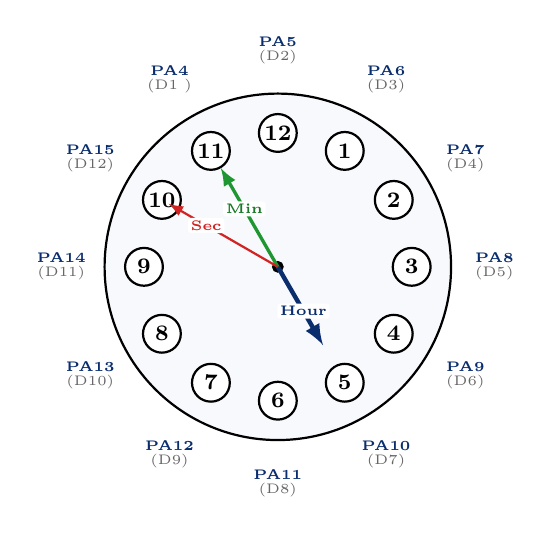
\begin{tikzpicture}[>=latex, scale=1.0, every node/.append style={transform shape}]
    % Outer dial ring
    \draw[thick, fill=codebg] (0,0) circle (2.2cm);
    \draw[thick, fill=black] (0,0) circle (0.06cm);

    % 12 radial positions: numeral inside dial, pin and diode stacked outside
    \foreach \angle/\hour/\pin/\d in {
      90/12/PA5/D2, 60/1/PA6/D3, 30/2/PA7/D4, 0/3/PA8/D5,
      -30/4/PA9/D6, -60/5/PA10/D7, -90/6/PA11/D8, -120/7/PA12/D9,
      -150/8/PA13/D10, -180/9/PA14/D11, -210/10/PA15/D12, -240/11/PA4/D1
    } {
      \coordinate (P) at (\angle:1.70cm);
      \coordinate (L) at (\angle:2.75cm);
      \draw[fill=white, draw=black, thick] (P) circle (0.24cm);
      \node[font=\footnotesize\bfseries] at (P) {\hour};
      \node[font=\tiny, align=center] at (L) {\textbf{\color{darkblue}\pin}\\[-1pt]\color{gray!80!black}(\d)};
    }

    % Example hands at 05:59:50
    % Hour hand: 5 o'clock (-60 deg)
    \draw[->, ultra thick, color=darkblue] (0,0) -- (-60:1.15cm);
    \node[font=\tiny\bfseries, color=darkblue, fill=white, inner sep=1pt, rounded corners=1pt] at (-60:0.65cm) {Hour};
    % Minute hand: 59 min => pos 11 (120 deg)
    \draw[->, very thick, color=signalgreen] (0,0) -- (120:1.45cm);
    \node[font=\tiny\bfseries, color=signalgreen!80!black, fill=white, inner sep=1pt, rounded corners=1pt] at (120:0.85cm) {Min};
    % Second hand: 50 sec => pos 10 (150 deg)
    \draw[->, thick, color=signalred] (0,0) -- (150:1.60cm);
    \node[font=\tiny\bfseries, color=signalred, fill=white, inner sep=1pt, rounded corners=1pt] at (150:1.05cm) {Sec};
  \end{tikzpicture}
  \vspace{-0.8em}
  \caption{12-LED analog clock dial schematic and hand vector representation}
  \label{fig:clock_vector}
\end{figure}

\setlength{\abovedisplayskip}{3pt}
\setlength{\belowdisplayskip}{3pt}
\setlength{\abovedisplayshortskip}{1pt}
\setlength{\belowdisplayshortskip}{1pt}

\paragraph{Mathematical Hand Discretization}
The hour, minute, and second values are quantized into 12 discrete angular sectors:
\begin{equation}
  \text{pos}_{\text{hour}} = \text{hour} \pmod{12}, \quad
  \text{pos}_{\text{minute}} = \lfloor \text{minute} / 5 \rfloor, \quad
  \text{pos}_{\text{second}} = \lfloor \text{second} / 5 \rfloor
\end{equation}

\paragraph{Overlapping Hands and Pairwise Distinct Conditions}
A fundamental physical property arises from mapping three continuous time hands onto 12 shared discrete indicators:
\begin{itemize}[leftmargin=*,itemsep=0pt,topsep=1pt,partopsep=0pt,parsep=0pt]
  \item \textbf{Three Distinct Positions:} Exactly \textbf{3 distinct LEDs} are illuminated if and only if the three hand positions are pairwise distinct:
  \begin{equation}
    \text{pos}_{\text{hour}} \ne \text{pos}_{\text{minute}} \quad \text{and} \quad \text{pos}_{\text{minute}} \ne \text{pos}_{\text{second}} \quad \text{and} \quad \text{pos}_{\text{hour}} \ne \text{pos}_{\text{second}}
  \end{equation}
  \item \textbf{Two Hands Coincide:} If exactly two hands occupy the same 5-minute sector (e.g., at $12:00:15$, $\text{pos}_{\text{hour}} = 0$ and $\text{pos}_{\text{minute}} = 0$, while $\text{pos}_{\text{second}} = 3$), the bitwise OR union excites only 2 pins, so \textbf{exactly 2 distinct LEDs} are illuminated.
  \item \textbf{All Three Hands Coincide:} At times such as \textbf{$01:05:05$} (or $12:00:00$), all three hands evaluate to the exact same position ($\text{pos}_{\text{hour}} = 1 \pmod{12} = 1$, $\text{pos}_{\text{minute}} = \lfloor 5/5 \rfloor = 1$, $\text{pos}_{\text{second}} = \lfloor 5/5 \rfloor = 1$). The bitwise union yields a single active pin, illuminating \textbf{only 1 distinct LED}.
\end{itemize}
\noindent Therefore, three time values correspond to \textbf{fewer than three distinct illuminated LEDs whenever two or more hands overlap}.

\paragraph{Atomic Port Manipulation via BSRR}
In \texttt{displayClock()}, active LED bitmasks combine with bitwise OR, and inactive LEDs are isolated:
\begin{align}
  \text{on\_pins} &= \text{clock\_pins}[\text{pos}_{\text{hour}}] \mid \text{clock\_pins}[\text{pos}_{\text{minute}}] \mid \text{clock\_pins}[\text{pos}_{\text{second}}] \\
  \text{off\_pins} &= \text{CLOCK\_LED\_MASK} \ \& \ (\sim\text{on\_pins})
\end{align}
The entire 12-pin port configuration is applied in a single atomic instruction to the Bit Set/Reset Register \cite{rm0008}:
\begin{equation}
  \texttt{GPIOA->BSRR} = (\text{uint32\_t})\text{off\_pins} \mid ((\text{uint32\_t})\text{on\_pins} \ll 16)
\end{equation}
Because the \texttt{BSRR} high-half resets pins low (turning LEDs ON) and low-half sets pins high (turning LEDs OFF) simultaneously, the clock updates without intermediate glitch states.

\paragraph{Verbatim Clock Implementation Source Code}
The listings below present the verbatim display driver and real-time execution loop from \texttt{Lab1\_e10/Core/Src/main.c}:

\begin{lstlisting}[caption={[Clock display and atomic BSRR driver]{Clock display and atomic BSRR driver (Lab1\_e10/Core/Src/main.c)}},label={lst:ex10_driver},basicstyle=\fontsize{6.8pt}{7.5pt}\ttfamily,lineskip=0pt,aboveskip=0pt,belowskip=0pt]
#define CLOCK_LED_MASK ((uint16_t)0xFFF0U)

static const uint16_t clock_pins[12] =
{
    GPIO_PIN_5,
    GPIO_PIN_6,
    GPIO_PIN_7,
    GPIO_PIN_8,
    GPIO_PIN_9,
    GPIO_PIN_10,
    GPIO_PIN_11,
    GPIO_PIN_12,
    GPIO_PIN_13,
    GPIO_PIN_14,
    GPIO_PIN_15,
    GPIO_PIN_4
};

static void displayClock(uint8_t hour, uint8_t minute, uint8_t second)
{
    const uint16_t on_pins = clock_pins[hour % 12U]
                           | clock_pins[minute / 5U]
                           | clock_pins[second / 5U];
    const uint16_t off_pins = CLOCK_LED_MASK & (uint16_t)~on_pins;

    /* Update all hands together; leave PA0-PA3 unchanged.
     * Low half sets OFF pins high; high half resets ON pins low.
     * Overlapping hands naturally share the same LED.
     */
    GPIOA->BSRR = (uint32_t)off_pins | ((uint32_t)on_pins << 16U);
}
\end{lstlisting}

\begin{lstlisting}[caption={[Real-time tick loop with rollover]{Real-time tick loop with rollover management (Lab1\_e10/Core/Src/main.c)}},label={lst:ex10_loop},basicstyle=\fontsize{6.8pt}{7.5pt}\ttfamily,lineskip=0pt,aboveskip=0pt,belowskip=0pt]
    /* Initial time: 05:59:50 */
    uint8_t hour = 5;
    uint8_t minute = 59;
    uint8_t second = 50;
    uint32_t previous_tick = HAL_GetTick();

    displayClock(hour, minute, second);

    while (1)
    {
        /* Unsigned subtraction also handles the HAL tick wrapping.
         * Fixed deadlines avoid adding loop execution time each second.
         */
        while ((uint32_t)(HAL_GetTick() - previous_tick) >= 1000U)
        {
            previous_tick += 1000U;
            if (++second >= 60U)
            {
                second = 0;
                if (++minute >= 60U)
                {
                    minute = 0;
                    if (++hour > 12U)
                    {
                        hour = 1;
                    }
                }
            }
            displayClock(hour, minute, second);
        }
        HAL_Delay(1);
    }
\end{lstlisting}

\paragraph{Time-Base Generation and Rollover Execution}
Starting at $05:59:50$, the system executes for 10 seconds, reaching a cascading rollover: at second 60, \texttt{second} resets to 0, \texttt{minute} rolls from 59 to 0, and \texttt{hour} advances from 5 to 6 ($06:00:00$). At $06:00:00$, the hour hand maps to position 6 (PA11), while minute and second hands coincide at position 0 (PA5), illuminating exactly 2 distinct LEDs. This behavior is established from source analysis.

% ==============================================================================
% SECTION 4
% ==============================================================================

\section{Repository Artifact Links}
Each design module is committed in the project repository:
\begin{itemize}[leftmargin=*,itemsep=1pt]
  \item \textbf{Ex 1 Proteus Project:} \href{https://github.com/tapstoptap/microcontroller-261/raw/77b62e494c47b4563374bc61c562bf9e5548d887/Proteus_Project/Lab1_e1/Lab1_e1.pdsprj}{\texttt{Proteus\_Project/Lab1\_e1/Lab1\_e1.pdsprj}}
  \item \textbf{Ex 2 Proteus Project:} \href{https://github.com/tapstoptap/microcontroller-261/raw/77b62e494c47b4563374bc61c562bf9e5548d887/Proteus_Project/Lab1_e2/Lab1_e2.pdsprj}{\texttt{Proteus\_Project/Lab1\_e2/Lab1\_e2.pdsprj}}
  \item \textbf{Ex 3 Proteus Project:} \href{https://github.com/tapstoptap/microcontroller-261/raw/77b62e494c47b4563374bc61c562bf9e5548d887/Proteus_Project/Lab1_e3/Lab1_e3.pdsprj}{\texttt{Proteus\_Project/Lab1\_e3/Lab1\_e3.pdsprj}}
  \item \textbf{Ex 4 Proteus Project:} \href{https://github.com/tapstoptap/microcontroller-261/raw/77b62e494c47b4563374bc61c562bf9e5548d887/Proteus_Project/Lab1_e4/Lab1_e4.pdsprj}{\texttt{Proteus\_Project/Lab1\_e4/Lab1\_e4.pdsprj}}
  \item \textbf{Ex 5 Proteus Project:} \href{https://github.com/tapstoptap/microcontroller-261/raw/77b62e494c47b4563374bc61c562bf9e5548d887/Proteus_Project/Lab1_e5/Lab1_e5.pdsprj}{\texttt{Proteus\_Project/Lab1\_e5/Lab1\_e5.pdsprj}}
  \item \textbf{Ex 6 Proteus Project:} \href{https://github.com/tapstoptap/microcontroller-261/raw/77b62e494c47b4563374bc61c562bf9e5548d887/Proteus_Project/Lab1_e6/Lab1_e6.pdsprj}{\texttt{Proteus\_Project/Lab1\_e6/Lab1\_e6.pdsprj}}
  \item \textbf{Ex 10 Proteus Project:} \href{https://github.com/tapstoptap/microcontroller-261/raw/77b62e494c47b4563374bc61c562bf9e5548d887/Proteus_Project/Lab1_e10/Lab1_e10.pdsprj}{\texttt{Proteus\_Project/Lab1\_e10/Lab1\_e10.pdsprj}}
\end{itemize}

% References
\vspace{0.6em}
\begin{thebibliography}{99}
\small
\setlength{\itemsep}{1pt}
\bibitem{rm0008}
STMicroelectronics, \textit{RM0008 Reference Manual: STM32F101xx, STM32F102xx, STM32F103xx, STM32F105xx and STM32F107xx advanced Arm-based 32-bit MCUs}, Rev.~21, 2021.

\bibitem{ds15060}
STMicroelectronics, \textit{STM32F103x4, STM32F103x6 Low-Density Performance Line ARM-Based 32-Bit MCU Datasheet}, DocID 15060 Rev.~10, 2020.

\bibitem{um1850}
STMicroelectronics, \textit{UM1850 User Manual: Description of STM32F1 HAL and low-layer drivers}, Rev.~5, 2021.

\bibitem{nhanlab}
Le~Trong Nhan, \textit{Lab 01: LED Animations --- Microcontroller Laboratory Manual}, Department of Computer Engineering, Faculty of Computer Science and Engineering, Ho Chi Minh City University of Technology (HCMUT), pp.~20--23.

\bibitem{proteusvsm}
Labcenter Electronics Ltd., \textit{Proteus VSM for ARM Cortex-M3 Simulation Guide}, Version 8.13, 2021.

\bibitem{githubrepo}
N.~M.~Phuc, \textit{Microcontroller Course Laboratory Code Repository}, GitHub repository, commit \texttt{77b62e4}, 2026. \url{https://github.com/tapstoptap/microcontroller-261.git}.
\end{thebibliography}

\end{document}
